\documentclass[12pt,a4paper]{book}
\usepackage[T1]{fontenc}
\usepackage[utf8]{inputenc}
\usepackage{cite}
\usepackage{amsmath,mathtools,breqn,amsfonts, amsthm, mathrsfs, amssymb}
\usepackage[margin=3cm,letterpaper]{geometry} % decreases margins
\usepackage{comment}
\usepackage{hyperref}
\usepackage{color}
\usepackage{listings}
\usepackage{caption}
\usepackage{enumitem}
\usepackage{graphicx,caption}
\usepackage[toc,page]{appendix}
\usepackage{algorithm, algpseudocode}
\usepackage{makecell}
\usepackage[demo]{subcaption}

\definecolor{green}{RGB}{60,179,113}
\definecolor{violet}{RGB}{153,50,204}
\definecolor{blue}{RGB}{65,105,225}
\definecolor{gray}{RGB}{128,128,128}
\definecolor{red}{RGB}{255,100,100}
\definecolor{lightpurple}{RGB}{215,189,226}
\definecolor{lightgreen}{RGB}{171,235,198}
\definecolor{yellow}{RGB}{249,231,159}
\definecolor{pink}{RGB}{253,175,172}
\definecolor{lightblue}{RGB}{174,214,241}

% set up the colors for different kind of references
\hypersetup{
	colorlinks = true,
	linkcolor  = violet,
	citecolor  = green 
}

\lstset{
	language=C,
	aboveskip=3mm,
	belowskip=3mm,
	xleftmargin=5mm,
	showstringspaces=false,
	columns=flexible,
	basicstyle={\small\ttfamily},
	numbers=left,
	numberstyle=\tiny\color{gray},
	keywordstyle=\color{blue},
	morekeywords={bool},
	commentstyle=\color{green},
	stringstyle=\color{violet},
	breaklines=true,
	breakatwhitespace=true,
	tabsize=4,
	frame=tlrb
}

\newcommand\defeq{\stackrel{\mathclap{\normalfont\mbox{\tiny def}}}{=}}

\newcommand{\st}{\hspace{2px}.\hspace{2px}}

\theoremstyle{definition}
\newtheorem{defn}{Definition}

\raggedbottom

\begin{document}
	%\frontmatter
	
	\pagenumbering{gobble}
	\begin{titlepage}
		\begin{center}
			\vspace*{1cm}
			
			\Huge
			\textbf{\Huge Detecting Microarchitectural Attacks}
			
			\vspace{0.3cm}
			\LARGE \textsc{Draft}
			
			\vspace{1.5cm}
			
			\large Author: \textit{Magdalena M. Solitro}
			
			\vfill
		\end{center}
	\end{titlepage}
	
	\tableofcontents
	
	\mainmatter
	
	\chapter*{Notation}\label{chapter:notation}
	
	% ridefinisco lo spazio tra righe
	\renewcommand{\arraystretch}{2.0}
	% aumento lo spazio tra colonne
	\setlength{\tabcolsep}{25pt}
	\begin{tabular}{l l}
		$\forall$ & \makecell[l]{universal quantification, it is read "for all" and it expresses a \\predicate that can be satisfied by \textit{every member} of a domain\\ of discourse} \\
		$\exists$ & \makecell[l]{existential quantification, it is read "it exists" and it expresses \\a predicate that is satisfied by \textit{at least one member} of a domain\\ of discourse} \\
		$\in$ & set belonging \\
		$p$ & a generic program \\
		$\mathcal{L}$ & a generic programming language \\
		$\mathcal{P}$ & \makecell[l]{a semantic property, i.e. the set of all programs that satisfy a\\certain property} \\
		$\emptyset$ & the empty set \\
		$\vee$ & logical "or"\\
		$\wedge$ & logical "and"\\
		$A \Longrightarrow B$ & $A$ implies $B$ (if $A$, then $B$)\\
		$A \Longleftarrow B$ & $B$ implies $A$ (if $B$, then $A$)\\
		$A \Longleftrightarrow B$& $A$ implies $B$ and $B$ implies $A$ ($A$ if and only if $B$)\\
	\end{tabular}\\

	\chapter{Introduction}\label{chapter:intro}
	Within the harware products market, companies such as Intel, AMD, Nvidia, and so on, strive to produce faster, smaller, energy-efficient chips to beat the competition and grant themselves the biggest market share. However, achieving the best results in every aspect is concretely infeasible: for instance, highly performing devices tend to consume a greater amount of power, while chips must trade small dimensions with memory capacity. Therefore, the main challenge is to reach an acceptable trade-off between all the different aspects that influence the performance of a device.

	Speed is a hot topic when it comes to CPU design: most users want their computer to go \textit{fast}, and to satisfy this request, engineers keep coming up with all sorts of expedients. One of the most effective dodges to achieve higher performances is \textit{speculative execution} (also known as \textit{transient execution}), which consists in retrieving in advance from the main memory instructions that have a higher chance to be executed, to reduce the time that the processor spends idle, waiting for the instruction and the data involved to be loaded in the cache. 
	This comes useful in presence of conditional branches: since it's impossible to statically infer what branch is going to be selected, the CPU uses statistical information about previous executions to \textit{speculate} about how the conditional expression will be evaluated, and thus what set of instruction will need to be retrieved.
	
	The introduction of speculative execution successfully improved the CPU performances, but at the same time it introduced some unforeseen security flaws that were discovered only after these processors had already been installed in thousands of machines: Flush+Reload \cite{Yarom2014}, Spectre \cite{Kocher2019}, Meltdown \cite{Lipp2018}, Spoiler \cite{Islam2019} are the names of some vulnerabilities that exploit a chache side-channel opened by transient execution to expose potentially secret information.
	
	Starting from 2018, the year in which these attacks were disclosed, many efforts have been made to patch them, but ditching speculative execution completely was never an option, as the impact on performances would have been too great. Instead, a series of strategies have been engineered to at least mitigate its consequences on the security of programs. Besides this, another problem needed to be addressed was how to figure out whether a software was vulnerable or not to such side-channel attacks. One way to do it is to use \textit{static analysis} to inspect the code before its execution and detect specific patterns or possible execution paths that can lead to a data leakage. While these techniques are not guaranteed to always provide the correct result, they are considered to be highly reliable to verify the properties of a program.
	
	In this thesis, we target a specific security vulnerability, Spectre, and we use static analysis techniques to inspect popular software libraries to verify if they can suffer from Spectre-like attacks. We chose specific libraries from OpenSSL\footnote{\url{https://www.openssl.org/}}, a project that aims to provide robust, general-purpose software to ensure secure communication over the network. We decided to test OpenSSL for many reasons: it's open-source, it's written in a language that lend itself well for the analysis that we plan to carry out, and it's one of the most widely used libraries at the moment. Furthermore, OpenSSL notoriously suffered from various security bugs since its earliest versions (one of the most serious ones was Heartbleed\footnote{\url{https://heartbleed.com/}}, disclosed in April 2014), so I thought it would be interesting to see if it's a fertile ground for attacks based on speculative execution. More precisely, in this thesis we submit selected OpenSSL libraries to two different static analysis tools, that employ different detection strategies: one dates back to 2020 and is considered to be a state-of-the-art tool, while the other one is more recent and uses an uncommon, yet promising approach that was not seen in any other analysis tool for Spectre detection. At the end of our study, we will not only test whether OpenSSL is immune or not to Spectre-like vulnerabilities, but we will also compare these two tools from different points of view, to evaluate their effectiveness and their performances.
	
	The thesis is structured as follows: Chapter \ref{chapter:static_analysis} covers the main notions about static analysis and its theoretical basis, along with a focus on some practical strategies employed by one of the tools that we will use later; Chapter \ref{chapter:spectre} is instead focused on Spectre and will present not only the microarchitectural details that allow to exploit the side effects of speculative execution, but will also provide an in-depth description of all the Spectre variants currently known. We then proceed with Chapter \ref{chapter:verification}, that contains the core of this work: it describes the tools selected to test OpenSSL, providing an overview of the strategies they enforce to detect Spectre and presenting the experimental results obtained by submitting the selected libraries to these tools. The rest of the thesis is dedicated to the appendices, where we cover notions on complexity theory, deep learning, and cryptography that can come useful to those readers who are not familiar with the topics for comprehending various part of this thesis.
	
	\chapter{Static analysis for cybersecurity}\label{chapter:static_analysis}
	Static analysis is a set of automated techniques used to inspect a program to check whether it satisfies certain properties, without executing it. The origins of static analysis date back to the Seventies and it was initially developed to speed up the compilation process. Nowadays, these techniques are used for a multitude of purposes, such as program verification, synthesis of optimised code, and certification of critical software applications \cite{Rival2020}. 
	
	This chapter will provide an insight on the theoretical principles and practical approaches of static analysis, with particular attention to the cybersecurity perspective. Some of the question concerning safety and security that we can tackle with static analysis are, for example: will the software crash under certain circumstances? Will specific inputs give illicit access to information that shouldn't be disclosed? Does the software accomplish \textit{exactly} what it is programmed for or will there be undesired side effects? We can try to give an answer to these questions through intensive testing, but this approach is destined to be a coarse approximation of the correct answer: the domain of possible inputs that need to be examined is often far too broad to be tested in a reasonable amount of time and selecting a small subset of inputs is likely to leave out those few that can cause a malfunctioning. In addition to that, nowadays computer programs are behind the correct functioning of safety-critical systems, such as industrial machinery or avionics: in these contexts, where unexpected behaviours can likely cause serious injuries or even death, the analysis of the program cannot be left to inaccurate methods. These are just a couple of reasons that highlight the necessity of techniques that allow us to verify quickly and precisely the properties of a program.
	
	We begin our dive into static analysis by firstly providing the theoretical arguments on which this field is based and then we will move on to describe some modern strategies to carry out the analysis. All the notation used throughout this chapter is summarised at the beginning of this thesis, in the chapter "Notation".
	\section{Theoretical foundations}
	The goals of static analysis are ambitious, because it aims to provide tools that can deliver the following advantages:
	\begin{itemize}
		\item \textbf{Speed:} the possibility of using methods to analyse code quickly implies being able to perform more controls, more frequently; 
		\item \textbf{Automation:} being able to check the properties of a program automatically relieve humans from a cumbersome and error-prone process;
		\item \textbf{Precision:} static analysis can detect flaws that appear only very rarely during execution, and thus would be hard to spot through simple testing.
	\end{itemize}
	These objectives can be partially achieved, although not entirely:  static analysis is not infallible, which means that it does not always provide the correct results. To be more precise, the effectiveness of static analysis has to confront some intrinsic limits of computation, namely the undecidability of the \textit{Halting problem} and \textit{Rice's theorem}. 
	\theoremstyle{theorem}
	\newtheorem{thm}{Theorem}
	\begin{thm}[Halting problem] Let $\mathcal{L}$ be the set of all programs that can be written in a certain language, and let $p$ be one of such programs. 
		
		The halting problem consists in finding an algorithm \texttt{halt} such that,  
		\[
		\forall\hspace{2px}p\in\mathcal{L}\st\texttt{halt(p)} = true \Longleftrightarrow p\text{ terminates}
		\]
		The halting problem is not computable: an algorithm such as \texttt{halt} does not exist, as proved simultaneously by Alonso Church \cite{Church1936} and Alan Turing \cite{Turing1937} in 1936.
	\end{thm}
	This theorem provide an example of something that a program analysis tool cannot detect: no algorithm can decide whether a program, written in any language, will terminate or not.
	
	There is another theoretical result, that provides an even stronger statement on what we can prove about the properties of a program:
	\begin{thm}[Rice's Theorem] Let $\mathcal{L}$ be a Turing-complete language, and let $\mathcal{P}$ be a nontrivial semantic property of programs of $\mathcal{L}$. There exists no algorithm \texttt{SatP} such that,
		\[
		\forall\hspace{2px}p\in\mathcal{L}\st\texttt{SatP(p)} = true \Longleftrightarrow p\text{ satisfies the semantic property } \mathcal{P}. 	
		\]
	\end{thm}
	The notion of "nontrivial" mentioned in the theorem identifies those properties that either concern \textit{every} program in the language, or \textit{none}, therefore
	\[
	\mathcal{P}\text{ is trivial} \Longleftrightarrow \mathcal{P} = \mathcal{L} \vee \mathcal{P} = \emptyset
	\]
	Clearly, we are not interested in trivial properties, because there is really nothing to prove about them in a program!
	Intuitively, what Rice's theorem states is that, for \textit{any interesting property}, we cannot have an algorithm that is able to decide whether a certain program has that property or not. This sounds discouraging: the theorems mentioned above seem to destroy any hope of being able to prove anything interesting about programs. Luckily, this is not quite the case: while it is impossible to have an automated procedure that correctly detects a certain property in \textit{all} cases, it is perfectly possible that it does it \textit{sometimes}. This also means that it's impossible to construct a "perfect" static analysis tool, namely one that is always able to detect any (extensional) property of a program: this justifies the existance of a research field dedicated to static analysis.
	
	What we just said implies that the results provided by the algorithm will occasionally produce incorrect results, such as false positives and false negatives: the former refers to the detection of bugs that the program doesn't actually have, while the second one regards the failure of finding bugs that the code indeed has. False negatives are clearly a much bigger issue, because they lead to a false sense of security: for this reason, a good tool for static analysis should never fail to detect bugs, while it is allowed to output a false positive \cite{Gomes2009}. Another way around the limitation of Rice's Theorem is to give up complete automation, designing tools that require human intervention to compute the final result, accepting the risk of introducing mistakes in the computation of the final result.
	
	The desiderable properties of a program analysis tools can be formalised by means of two notions: \textit{soundness} and \textit{completeness}.
	
	\begin{defn}[Soundness]
		Let \texttt{analyse} be a program that tests whether another program has a certain property $\mathcal{P}$ and let $\mathcal{L}$ be a programming language. We say that the program \texttt{analyse} is \textbf{sound} with respect to $\mathcal{P}$ if the following condition is satisfied:
		\[
		\forall p \in \mathcal{L} \st \text{\texttt{analyse}}(p) = \text{\textbf{true}} \Longrightarrow p \text{ satisfies } \mathcal{P}
		\]
	\end{defn}
	In simple terms, a proof system is sound if all the statements it proves are actually true. A trivial \texttt{analysis} program that is guaranteed to be sound is the one that always returns false: by invalidating the premise, it makes the overall implication to be true, even though such analyser would clearly be of no utility.
	
	For the definition of completeness, we stick to the same notation.
	\begin{defn}[Completeness]
		We say that a program \texttt{analyse} is \textbf{complete} with respect to $\mathcal{P}$ if the following condition is satisfied:
		\[
		\forall p \in \mathcal{L} \st p \text{ satisfies } \mathcal{P} \Longrightarrow \text{\texttt{analyse}}(p) = \text{\textbf{true}} 
		\]
	\end{defn}
	As the definition suggests, a \textit{complete} analyser is one that is able to prove \textit{all} the properties that are satisfied by a program. More generally, a formal system is said to be complete with respect to a particular property, if every formula that satisfies that property is a theorem (i.e. can be proved) within the system.
	
	Also in this case, we can provide a trivial \texttt{analysis} program that is guaranteed to be complete, namely the one that always returns true. In fact, if the consequence is true, the overall implication will always evaluate to true, independently from the truth value of the premise.
	
	Soundness and completeness are two essential aspect of a correct analysis, but an inherent limit of computability prevents us from having both. This limit is a consquence of Gödel's Incompleteness Theorems, which essentially show that there is an intrinsic gap in mathematics between \textit{proof} and \textit{truth}. These theorems are extremely complex and profound, and thus we will not dive into their details, but the interested readers can find out more about the topic in \cite{Odifreddi1989}, \cite{Rogers1987}, \cite{Hinman2007}.
	\section{Practical approaches and related challenges}
	This section discusses the general concepts behind the approaches used by the tools discussed in Chapter \ref{chapter:verification}. The description should be considered as a high-level introduction whose aim is to give an idea of the mechanisms leveraged by these tools, but more accurate descriptions can be found in the papers cited throughout this section.
	\subsection{Taint analysis}\label{sec:taint}
	Taint analysis is a technique that involves labelling each variable supplied to the program by an untrusted source as \textit{tainted}, assuming that the untrusted source could be an adversary trying to attack the system  through that variable.
	Then, every variable in the program whose value is dependent from tainted variables is also marked as tainted. In this way, we can keep track of the propagation of tainted data in the following instructions and detect when this data is used in dangerous ways. Taint analysis can be used to identify parts of code vulnerable to Spectre: for instance, in a Spectre-PHT attack, certain values can be supplied repeatedly to a conditional branch to induce a misprediction. The following example shows a Spectre-PHT gadget where the tainted variables are marked in red:
	
	\vspace{3mm}
	\begin{minipage}{.6\textwidth}
	\begin{lstlisting}[escapechar=!]
int checkValue(int !\colorbox{red}{x}!){
	if(!\colorbox{red}{x}! < len(array1)){
		!\colorbox{red}{y}! = array2[array1[!\colorbox{red}{x}!] * 4096;
	}
	return y;
}
	\end{lstlisting}
	\end{minipage}

	The parameter \texttt{x} is supplied by the user, therefore is marked as tainted. The value of \texttt{y}, determined in line 3, depends on \texttt{x}, thus \texttt{y} becomes automatically tainted. This is an example of taint (dynamic) analysis \textit{based on data flow}, because it involves marking external taint data and tracking its propagation throughout the execution.
	
	This type of analysis can be used for vulnerability detection \cite{Newsome2005}, malware analysis \cite{Bayer2009} \cite{Yin2007}, and web applications \cite{Balzarotti2008} \cite{NguyenTuong2005}, and can be applied both statically or dynamically.
	
	Dynamic taint analysis can be based either on \textit{data flow} (the example above is an instance of this approach) or on \textit{control flow}. The latter involves constructing a control flow graph (CFG) of the program, by examining the branching instructions that govern the execution of the code \cite{Dai2018}.
	
	\subsubsection{Challenges in taint analysis}
	The main issues that taint analysis encounters are \textbf{under-tainting}, \textbf{over-tainting} and \textbf{state space explosion}. Let's start with the first one: under-tainting means that the analysis tool does not mark as tainted a data that was should be marked as such. This happens when the data is not arithmetically derived by an untrusted input or, more generally, is not linked to such input by an explicit instruction in the program, but is still influenced by it. This phenomenon causes the detection of \textbf{false negatives}, namely the tool recognises a piece of code as secure, even though it's not. A clever example of how this can occur is proposed in \cite{Newsome2005}:
	
	\vspace{3mm}
	\begin{minipage}{.4\textwidth}
	\begin{lstlisting}
if(x==0){ y=0; } 
else if (x==1){ y=1; } 
else if (x==2){ y=2; } 
...
	\end{lstlisting}
	\end{minipage}

	This conditional structure goes on in the form
	
	\vspace{3mm}
	\begin{minipage}{.3\textwidth}
	\begin{lstlisting}[mathescape=true]
if(x == $n$){ y = $n$; }
	\end{lstlisting}
	\end{minipage}

	The program is semantically equivalent to the following instruction:
	
	\vspace{3mm}
	\begin{minipage}{.15\textwidth}
	\begin{lstlisting}
y = x;
	\end{lstlisting}
	\end{minipage}

	A taint analysis will mark \texttt{y} as tainted in the last instruction, but not in the first example.
	
	The opposite problem is \textbf{over-tainting}, which leads to the detection of false positives: a piece of code can be evaluated as insecure, even in the absence of any feasible execution that taints a certain data. As already stated previously in this chapter, false positives are preferred to false negatives, since the latter can give a false sense of security and fail to notify potential vulnerabilities. One source of over-tainting can be a conservative extraction of the Control Flow Graph (CFG), which is defined as follows:
	\begin{defn}[Control Flow Graph (CFG)]
		A \textit{control flow graph (CFG)} is a directed graph $G=(V,E)$ in which nodes represent the program's instructions, while an edge $u \rightarrow v$ represents a possible flow from the instruction $u$ to the instruction $v$. This means that there exists at least one run of the program in which the execution of $u$ is followed immediately by the execution of $v$. The set $V$ of nodes contains also two special nodes: \textit{START}, that has no predecessors and from which every node is reachable, and \textit{END}, which has no successors and is reachable from every node.
	\end{defn}
	
	The construction of an accurate graph from the binary is often challenging, due to the difficulty in determining the targets of indirect branches and function calls. For this reason, tools such as oo7 \cite{Wang2019} use a conservative approximation of the CFG, which can contain more edges that expected.
	
	The last issue worth mentioning is the \textbf{state space explosion} (also known as path explosion), which can occur during the construction of the CFG or the Control Dependency Graph (CDG). The latter is defined as follows:
	
	\begin{defn}[Control Dependency Graph (CDG)]
		A \textit{control dependency graph (CDG)} \cite{Krinke2007} is a directed graph $G=(V,E)$ in which nodes represent the program's statements or expressions, while an edge $x\rightarrow y$ expresses the fact that the statement $x$ assigns a variable which is used in $y$, which means that the mere execution of $y$ depends on the value of the expression $x$. 
	\end{defn}
	The CDG is used by the analyser to keep track of how the tainted data affects the other variables in the program. However, as the complexity of the program increases, the size of these graphs grows exponentially and can become infeasible to analyse. This issue is also encountered in another popular approach, symbolic execution, which is discussed in the below. 
	\subsection{Symbolic execution}\label{sec:symbolic-exec}
	One way to test the behaviour of a program is to provide it with different, random inputs and observe the result of every execution. However, this approach presents a glaring limit: the domain of all the possible inputs can be extremely wide, if not infinite, which makes it infeasible to try all of them. One way around this obstacle is to use symbolic execution \cite{Baldoni2018} \cite{King76}: instead of using fully specified input values, we simultaneously explore multiple paths that a program can take under different inputs. This is possible by representing those inputs that cannot be determined statically under a symbol, namely an abstract value. Such inputs could be, for example, paramenters that must be provided by the user at run time.
	
	During the symbolic execution of a program, the analysis engine keeps track the following information:
	\begin{itemize}
		\item The next \textit{statement} to evaluate (\texttt{stmt}).
		\item A \textit{symbolic store} $\sigma$, that maps the variables of the program either with expressions over concrete values or with symbolic values.
		\item Some \textit{path constraints} $\pi$, namely "a formula that expresses a set of assumptions on the symbols due to branches taken in the execution to reach \texttt{stmt}" \cite{Baldoni2018}.
	\end{itemize}
	Different execution paths distinguish themselves by the assumptions that are made about the symbolic values. To give an idea about how this process works, consider the following piece of code:
	
	\vspace{3mm}
	\begin{minipage}{.4\textwidth}
	\begin{lstlisting}
int func(int a){
	int x = 1;
	bool y = true;
	if (a != 0){
		...
	}
}
	\end{lstlisting} 
	\end{minipage}

	At the beginning of the symbolic execution, the state maintained by the engine will be:
	\[
	(\textcolor{blue}{\texttt{stmt}}, \textcolor{violet}{\sigma}, \textcolor{green}{\pi}) = (\textcolor{blue}{\texttt{int x = 1}}, \textcolor{violet}{\sigma = \{a \mapsto \alpha_a\}}, \textcolor{green}{\pi = true})
	\]
	As you can see, \texttt{a} is a paramenter that can be known only at run time, as it is a user-supplied parameter. Therefore, the symbolic store will assign it to the symbolic value $\alpha_a$: this is a way of stating that, according to our current knowledge, \texttt{a} can assume any value in the range of integers, but we don't make any assumptions about it because it's not necessary (yet). $\pi$ is initially set to \textit{true} because we are currently making no assumption about the value of any symbol.
	
	The next step represent what happens after the (abstract) execution of \texttt{int x = 1}. The state is modified as follows, where the coloured elements are those that differ from the previous step:
	\[
	(\textcolor{blue}{\texttt{stmt}}, \textcolor{violet}{\sigma}, \pi) = (\textcolor{blue}{\texttt{bool y = true}}, \textcolor{violet}{\sigma = \{a \mapsto \alpha_a\, x \mapsto 1\}}, \pi = true)
	\] 
	Once the instruction on line 2 is executed, the symbolic store can map the variable \texttt{x} with the \textit{concrete} value 1, which can be inferred statically.
	
	The next instruction involves a branch conditioned on the value of \texttt{a}, which is not known. Therefore, the symbolic execution engine produces two paths, one for $\alpha_a = 0$ and the other for $\alpha_a \neq 0$:
	\[
	(\textcolor{blue}{\texttt{stmt}}, \sigma, \textcolor{green}{\pi}) = (\textcolor{blue}{\texttt{if (a != 0)}}, \sigma = \{a \mapsto \alpha_a\, x \mapsto 1\}, \textcolor{green}{\pi = \{\alpha_a = 0\}})
	\]
	\[
	(\textcolor{blue}{\texttt{stmt}}, \sigma, \textcolor{green}{\pi}) = (\textcolor{blue}{\texttt{if (a != 0)}}, \sigma = \{a \mapsto \alpha_a\, x \mapsto 1\}, \textcolor{green}{\pi = \{\alpha_a \neq 0\}})
	\]
	Through this kind of branching, the symbolic execution evolves as a tree until the program has terminated or until we gained enough knowledge to determine whether the property of interest is satisfied or not.
	\subsubsection{Challenges in symbolic execution}
	The tree structure of a symbolic execution suggests that this kind of analysis suffers of the same issue that we have already encoutered with taint analysis, namely \textbf{path explosion} (or state space explosion): as the size of the program grows, the number of feasible paths grows exponentially, and can even be infinite if the program contains unbounded loop iterations. Although an exhaustive exploration of the state space is the only way to guarantee a sound and complete analysis, a partial exploration is sufficient in many scenarios to prove a certain property, thus the problem of path explosion can often be circumvented.
	
	Another problem of symbolic execution concerns \textbf{constraint solving}. As precisely stated in \cite{Baldoni2018}, "in a symbolic executor, constraint solving plays a crucial role in checking the feasibility of a path, generating assignments to symbolic variables, and verifying assertions". These constraints are expressed in a logical language and their truth value is evaluated by decision procedures called "constraint solvers". 
	Finding a solution for such formulas is notoriously an NP-complete problem: for this reason, one of the most popular approaches to constraint solving consists in mapping the formula to an instance of the boolean satisfiability problem (also known as SAT, see Appendix \ref{appendix:complexity}), a famous NP-complete problem for which many efficient algorithms have been developed. For those problems that cannot be easily mapped to SAT, we can use Satisfiability Modulo Theories (SMT), that generalize the SAT problem with supporting theories to capture more complex formulas. Even though some significant advances has been accomplished in recent years to optimise the search of a solution, complexity remains a major obstacle to the scalability of symbolic execution to large programs. Moreover, not even SMT solvers are powerful enough to handle constraints that involve certain operations, such as non-linear arithmetic, which prevents us from exploiting the advantages of optimised SMT solvers.
	
	\chapter{Spectre}\label{chapter:spectre}
	On January 2018, two major vulnerabilities affecting the vast majority of modern CPUs were disclosed, taking the names of \textit{Spectre} \cite{Kocher2019} and \textit{Meltdown} \cite{Lipp2018}. These two attacks were independently discovered by various researchers and were published in 
	two works, \cite{Kocher2019} and \cite{Lipp2018}, destined to leave a permanent mark in the field of cybersecurity. More precisely, \cite{Kocher2019} identified \textit{Spectre}, a family of attacks that leverage on an optimisation technique used in modern processors to read and write protected memory from a program's address space, while \cite{Lipp2018} describes \textit{Meltdown}, an attack able to bypass the privilege checks that usually prevent a user process to access regions of memory that are under the control of the operating system. Both are classified as \textit{cache side-channel attacks} and were found to affect Intel, ARM and AMD processors, present in the vast majority of desktops, laptops, cloud servers, and even smartphones\footnote{Source: \url{https://spectreattack.com/}}.
	
	This chapter is focused on Spectre, which is classified as an \textit{access-driven cache side-channel attack}, as it is based on the adversary's ability to monitor cache accesses made by the victim and measuring the time difference between a cache access and a memory access.
	
	This chapter provides all the background notions that are needed to comprehend the mechanism of a Spectre attacks. Furthermore, it contains a complete overview of all the variants of the attacks that are currently known, describing what microarchitectural data structure they exploit and how the attack is carried out.
	\section{Background}
	This section deals with all the background concepts that lie at the basis of Spectre, in particular speculative execution and cache side channels. As stated in the pioneering work by Kocher et al. \cite{Kocher2019}, "Spectre attacks violate memory isolation boundaries by combining speculative execution with data exfiltration via microarchitectural covert channels."
	\subsection{Out-of-Order execution and micro-operations}\label{ooo-exec}
	When executing a program, the processor splits single assembly instructions in a series of lower-level operations called \textit{micro-operations} (also abbreviated as micro-ops or $\mu$-ops): this has the advantage of allowing the CPU to execute different part of the instructions in different moments, based on the current availability of the data \cite{Fog2021}. For example, consider the following piece of code, written in Intel syntax:
	
	\vspace{3mm}
	\begin{minipage}{.3\textwidth}
	\begin{lstlisting}
add eax, ebx
add [reg], eax
	\end{lstlisting}
	\end{minipage}

	The instruction on line 1 adds the content of two cache registers, \texttt{eax} and \texttt{ebx}. This means that the data will be immediately available to the CPU and thus this instruction doesn't need to be split in more than one $\mu$-op. The instruction on line 2, instead, is much different: it requires to (i) retrieve \texttt{[reg]}, namely the data located at the memory address stored in \texttt{reg}, then (ii) add it to the content of \texttt{eax}, and finally (iii) to write the result back to \texttt{[reg]}. Therefore, up to two memory accesses are needed to complete the instruction, but since these accesses are very time-consuming, the CPU splits the instructions into three $\mu$-ops (corresponding to the three step described), so that it can execute other tasks while it waits for the data to be accessible, avoiding to waste hundreds of clock cycles and thus speeding up the computation. This is precisely what is referred to as \textit{out-of-order execution}. This paradigm, however, comes with a challenge: when executing $\mu$-ops out of order, the CPU must establish whether there are dependencies between different instructions that can obstacle the completion of certain tasks.	For example, let's consider again the two assembly instructions written above: note that the addition on line 2 involves \texttt{eax}, which is modified by the previous addition. This means that the micro-operation (ii) can't be executed before the result of the previous addition is not stored in \texttt{eax}. To implement out-of-order execution successfully, the CPU uses a mechanism called \textit{memory disambiguation}, accurately described in \ref{sec:spectre-stl}, to detect and resolve this kind of dependencies. 
	
	\subsection{Speculative execution}\label{sec:speculative-exec}
	Speculative execution is an optimization technique where the CPU uses statistical information about the program execution to make guesses about the outcome of conditional branches or a data dependencies, and consequently decides to load data and execute certain micro-operations in advance. If the prediction is correct, the processor can benefit of the intermediate results and the data that loaded to speed up the execution of the following instructions. Otherwise, the CPU performs a rollback to the last correct state, discarding the intermediate results computed speculatively. It's imporatant to highlight that the effects of speculative execution are visible only at microarchitectural level until they are committed to the architectural state: the user doesn't have the perception that the execution flow is not strictly linear, and never sees the effect of incorrect predictions in the program's output. However, when a misprediction happen, the intermediate results and the data loaded preventively in cache remain there. This asymmetry between the microarchitectural state and what the user sees from the execution of the program gives space to the a type of attack vector known as \textit{cache side channel}, which is discussed in \ref{sec:cache-sc}.
	
	\subsection{Cache side channels}\label{sec:cache-sc}
	A cache side channel \cite{Zhang2017} is a type of attack vector that allows to infer secret variables by monitoring the state of the cache during the program execution. So far, three different kinds of cache side-channels have been identifies, each of which monitors different behaviours of the cache: time-driven \cite{Page2002}, trace-driven \cite{Page2002}, and access-driven.
	\paragraph{Time-driven side channels} In this case, the adversary keeps track of the execution time of the program and use that information to infer what data is loaded into the cache. 
	A typical example of timing attack targets the modular exponentiation function used in many public key cryptographic algorithm, included RSA. Modular exponentiation consists in raising a large number (i.e. the plaintext or the ciphertext) to a large exponent (i.e. the public key or the secret key respectively), which is extremely time consuming, since it requires to perform repeated multiplications using large integers. The subprocedure \texttt{square-and-multiply}, allows to do this computation efficiently:
	
	\vspace{3mm}
	\begin{minipage}{.6\textwidth}
	\begin{lstlisting}
square-and-multiply(M, e, N){
	R = 1
	for (i=0 to n-1){
		R = R^2 mod N
		if(e[i] == 1){ R = R * M mod N }
	}	
	return R
}
	\end{lstlisting}
	\end{minipage}

	where \texttt{M} is the message we want to encrypt (or decrypt), \texttt{e} is the exponent, \texttt{n} is the its length, \texttt{N} is the modulo, \texttt{R} is the result. As one can see, for each bit of the secret or public key \texttt{e}, the message is squared. If the current bit of the exponent is 1, then an additional multiplication is performed on the result: this means that, when the value of \texttt{e[i]} is 1, the computation on \texttt{R} takes longer to complete. This time difference could potentially be exploited to figure out which bits are set to 1 in the key, even though most systems nowadays employ some countermeasures to prevent it (for example, by adopting constant-time algorithms).
	\paragraph{Trace-driven side channels} In this attack, the adversary monitors the amount of power consumed during the execution. The power trace is a rich source of information, as it can reveal not only when certain operations are performed, but also what data is being used at each stage of the computation. The attacks carried out through this vector are also known as \textit{power analysis} attacks and they proved to be very effective: for example, numerous attacks of this kind have been successfully conducted on AES, the standard algorithm for simmetric encryption, to exfiltrate entire bytes of the symmetric key \cite{Buchanan2017} \cite{Mangard2003} \cite{Mangard2010} \cite{Oswald2004}. The attack is performed collecting a large number of power traces, on which the adversary performs different statistical analyses that can reveal the data dependency between the power consumption and the execution time. This attack style is known as \textit{Differential} Power Analysis (DPA), to distinguish it from \textit{Simple} Power Analysis (SPA), where the attacker needs only one single trace and tries to deduce information about the secret key from it.
	\paragraph{Access-driven side channels} 
	Access-driven attacks, like time-driven ones, leverage on time measurements to unveil the value of some secret information. However, they rely on a much finer kind of measurement: while time-driven attacks are based on the execution time of the whole program, access-driven ones exploit "the ability to
	detect whether a cache line has been evicted, or not, as the primary
	mechanism for mounting an attack" \cite{Neve2007}. From this point of view, this attack requires a much finer measurement capacity. A famous example of how to concretely exploit the timing information is \textsc{Flush$+$Reload} \cite{Yarom2014}, an attack that relies on sharing pages between the attacker and the victim processes. \textsc{Flush$+$Reload} can be summarised through the following steps: the adversary's goal is to verify whether the victim uses a secret piece of data $d$. To accomplish this, the adversary's process evicts the cache line containing $d$ and waits a certain amount of time, to give the victim the opportunity of using $d$, in case they need it. Then the attacker reloads the memory line and measures the time to load it: if the victim accessed $d$ during the latency time, the reload will be very quick, because $d$ was already brought back to the cache. Otherwise, $d$ is still in the main memory and the reloading time will be significantly longer, indicating that the victim did not access $d$ during the latency. Figure \ref{fig:flush-reload}, taken from the paper that first described the attack \cite{Yarom2014}, can help clarifying these concepts.  
	\begin{figure}[h!]
		\centering
		\includegraphics[scale=0.3]{../imgs/flush+reload}
		\captionsetup{width=.7\linewidth}
		\caption{\textsc{Flush+Reload} time measurement \cite{Yarom2014}. (A) and (B) represent the main cases described above. (C), (D), (E) are more peculiar cases.}
		\label{fig:flush-reload}
	\end{figure}
	One of the assumptions that must hold to carry out such attacks successfully is that the adversary must share the cache space with the victim.
	
	\section{Spectre variants}\label{sec:spectre-var}
	As mentioned at the beginning of this chapter, the term "Spectre" on itself does not identify a single attack, but a \textit{family} of attacks, all united by the same common denominator: they maliciously influence the speculative execution of a program to exfiltrate confidential information. Different version of Spectre can be carried out through the exploitation of different microarchitectural behaviours. The purpose of this section is to present the four main variants of Spectre, describing what vulnerability they take advantage of and in how they differ from each other.
	\subsection{Spectre-PHT (Pattern History Table)}\label{sec:spectre-pht}
	Spectre-PHT \cite{Kocher2019}\cite{Canella2019}\cite{Evtyushkin2018}, also known as variant 1 or Bound Check Bypass, was one the first attack of the Spectre family to be discovered. As the name suggests, this version targets the Pattern History Table (PHT) to trigger a branch misprection.
	\paragraph{Pattern History Table (PHT)} The Pattern History Table \cite{Fog2021} is a data structure used by the branch predictor to guess the outcome of a conditional branch before the value of the guard is fully determined. Intuitively, during the execution of a program, the CPU keeps track of the last $N$ outcomes of a conditional branch in the \textit{branch history register}. The outcomes are encoded as a bitstring of length $N$, where a 1 indicates an execution where the guard expression evaluated to true, while a 0 represents the opposite case. The content of the branch history buffer is used to point at a specific entry of the Pattern History Table. The PHT contains $2^N$ entries, i.e. as many entries as all the possible sequences of $N$ outcomes; each entry in
	the contains a 2-bit saturating counter, namely a finite-state automaton that decides the probability of a certain outcome. The branch history register is used for choosing which of the four counters to use.
	
	\paragraph{The attack} By poisoning the PHT, the adversary can induce the branch predictor to make a wrong guess about the direction of the conditional branch and perform both reading and writing operations in memory parts they shouldn't have the right to access. To clarify this concept, I propose a couple of examples, taken from \cite{Canella2019}: the first one, illustrated below, is one of the most well-known Spectre gadgets.
	
	\vspace{3mm}
	\begin{minipage}{.5\textwidth}
	\begin{lstlisting}
if(x < len(array1)) {
	y = array2[array1[x] * 4096]
}
	\end{lstlisting}
	\end{minipage}
	
	Note that the index we use to access \texttt{array2} is multiplied by 4096. The reason is that the usual cache block size is 64 bytes, so by using indexes in the form \texttt{[k * 4096]} we avoid having two elements used in the program falling into the same cache block.
	The conditional instruction allows reading a value from \texttt{array2} only if \texttt{x} represents a valid index. However, after repeatedly executing the conditional branch with a value of \texttt{x} that satisfies the guard, the branch predictor will forecast that the expression \texttt{x < len(array1)} evaluates to true and thus will execute the assignment on line 2 in advance. When the adversary supplies an invalid value for \texttt{x}, the CPU will performe an \textit{out-of-bounds memory access}, loading in the cache a value for \texttt{y} that shouldn't be accessed.
	
	The same effect can be exploited to perform a write operation on the array, as shown in the following piece of code:
	
	\vspace{3mm}
	\begin{minipage}{.5\textwidth}
	\begin{lstlisting}
if (x < len(array)) { 
	array[x] = value; 
}
	\end{lstlisting} 
	\end{minipage}
 
	Just as the described above, the attacker can "train" the CPU to guess a certain outcome of the branching instruction and then exploits the misprection caused by the provision of an invalid value of \texttt{x} to write on a protected location.
	\subsection{Spectre-BTB (Branch Target Buffer)}\label{sec:spectre-btb}
	Spectre-BTB \cite{Kocher2019} \cite{Canella2019}, also known as variant 2 or Branch Target Injection, affects the Branch Target Buffer to deflect the transient execution to a mispredicted branch target. This attack was discovered simultaneously to variant 1 and exploits a similar mechanism.
	
	\paragraph{Branch Target Buffer (BTB)} The Branch Target Buffer \cite{Perleberg1989} is a data structure located in the cache, that stores a set of guesses for the target addresses of all jumps, both conditional and unconditional. The first time a jump instruction is executed, the target address that is reached gets stored in the BTB, so no speculation is made for the first jump. When the jump is executed again, a pointer to the BTB indicates the target address of the previous execution, allowing the CPU to fetch the  predicted instruction into the pipeline, but the true target will not be calculated until the jump reaches the execution stage. Once the jump is actually performed,the address predicted with the BTB is compared with the actual address taken by the jump: if they don't match, the guess was wrong, so the results are rolled back and the previous target address is replaced by the current one in the BTB.
	\paragraph{The attack} The logic that governs this variant is very akin to the one behind Spectre-PHT: both attacks target data structures that aim to anticipate the outcome of jump instructions, trying to influence the prediction about what is executed as a consequence of the jump.
	
	However, there is a significant difference between Spectre-PHT and Spectre-BTB: in the former, the execution flows along a restricted mispredicted path, i.e. the attacker can influence the branch predictor only in the choice of the branch to execute. The latter, instead, allows redirecting the control flow to an arbitrary destination, so that the execution can continue at a specific point chosen by the adversary. This location corresponds to a \textit{Spectre gadget}, namely "a code fragment whose speculative execution will transfer the victim’s sensitive information into a covert channel"\cite{Kocher2019}.
	
	\subsection{Spectre-RSB (Return Stack Buffer)}\label{sec:spectre-rsb}
	Spectre-RSB \cite{Maisuradze2018} \cite{Koruyeh2018} \cite{Canella2019}, also known as ret2spec, is a variant that exploits a data structure called Return Stack Buffer.
	
	\paragraph{Return Stack Buffer (RSB)}The Return Stack Buffer is a microarchitectural buffer used to predict return address of a function: whenever a call instruction is reached during the execution, the prediction of the return address is pushed on top of a stack. When the execution reaches the \texttt{return} point, the top entry of the stack is used to speculate about the return address location quickly. Meanwhile, the actual return address is fetched, possibly from the main memory, therefore it will be available after only after hundreds of clock cycles. Once the real return address is loaded, it gets compared with the address that was fetched from the RSB: if they match, all the result computed until that point can be committed and the overall execution time gains in speed.
	
	\paragraph{The attack} To describe Spectre-RSB attacks, we also refer to another kind of stack: the \textit{program stack}, namely a data structure that stores information about the active subroutines of a computer program.
	
	There are various ways in which the adversary can poison the RSB, all described in detail in \cite{Koruyeh2018}. One way to carry out the attack is to exploit the stack overfill or underfill: the RSB has a very limited size, which can vary between 4 and 24 entries, thus it saturates quickly. When this happens, the stack gets updated in a cyclic manner, namely the latest return address is pushed on the stack, the $n$-th entry is discarded and the $(n-1)$-th takes its place. As the functions progressively reach the \texttt{return} instruction, the entries of both the program stack and the RSB get popped, but at some point we reach the function whose value has been overwritten, causing an underfill of the RSB.
	
	The primary attack strategy is to directly pollute the RSB: the adversary can overwrite the return address on the program stack, so that the top entry represents the return address of the previous function. In this way, the address found on the program stack and the on top of the RSB will certainly mismatch. 
	
	Another way is to leverage on the \textit{speculative} pollution of the RSB. When functions are called during a speculative execution and a misspeculation happens, their results are rolled back and they are removed from the stack. However, the guessed return addresses remain in the RSB, providing the opportunity to push an address that points outside the address space accessible by the program without raising exceptions.
	
	\subsection{Spectre-STL (Store To Load)}\label{sec:spectre-stl}
	Spectre-STL \cite{Canella2019}, also known as variant 4 or Speculative Store Bypass, is a variant that exploits not only dependencies in the control flow, but also those in in the \textit{data flow}. More precisely, this version takes advantage of the memory disambiguation mechanism that is put in place by most moder processors.
	
	\paragraph{Memory disambiguation} Memory disambiguation\footnote{\url{https://en.wikipedia.org/wiki/Memory_disambiguation}} is a set of techniques used to execute memory access instructions out of order, without affecting the value of the final result. To justify the need of these techinques, I will present two examples, both taken from (Wikipedia):
	
	\vspace{3mm}
	\begin{minipage}{.5\textwidth}
	\begin{lstlisting}
add $1, $2, $3      # R1 <= R2 + R3
add $5, $1, $4      # R5 <= R1 + R4
	\end{lstlisting}
	\end{minipage}
	
	The code above shows two micro-operations that perform simple additions. The result of the second instruction depends on the result of the first one, since the value of register R1 is computed in line 1 and then R1 is used as operand for the addition in line 2. This is a case of \textit{static} dependence, because the sources and destinations of the operations are registers. The processor can easily spot this dependence and decide an order of execution where the first addition is performed before the second one, so that the result is consistent with a sequential execution.
	
	However, "complications arise when the dependence is not statically determinable". Consider the following code snippet:
	
	\vspace{3mm}
	\begin{minipage}{.5\textwidth}
	\begin{lstlisting}
store $1, 2($2)      # Mem[R2+2] <= R1
load  $3, 4($4)      # R3 <= Mem[R4+4]
	\end{lstlisting}
	\end{minipage}

	In this case, the location of the operand is indirectly specified by means of a register, rather than directly defined in the instruction encoding itself. As clearly stated \href{https://en.wikipedia.org/wiki/Memory_disambiguation}{here}, "the microprocessor cannot statically determine, prior to execution, if the memory locations specified in these two instructions are different, or are the same location, because the locations depend on the values in R2 and R4". As a consequence, it is not possible to determine at compile time whether these two instructions can be executed in a different order or not: this is known as \textit{ambiguous} dependence. Detecting and resolving ambiguous dependencies require more sophisticated techniques than static dependency, and this is where the memory disambiguation mechanism comes into play.
	
	To further improve the performances, some processor support a technique called \textbf{memory dependence prediction}, which is analogous to branch prediction, that leaves room for a Spectre attack. This method aims at predicting the true dependencies between store and loads, in order to speculatively execute certain memory accesses out of order without affecting the final result of the computation. Similarly to the other variants, the guesses of the memory dependence predictor must be validated or discarded later in the pipeline, when the memory disambiguation system takes action and determines whether the loads and store where correctly executed.
	\paragraph{The attack} Spectre-STL exploits the prediction mechanisms to read a value from a protected address. The core idea of the attack leverages on the saw called \textit{RAW hazard}: "RAW" stands for "Read-After-Write" and it indicates a data dependency where a load operation reads a value from a memory location that was subjected to a store operation in a previous instruction. A RAW-hazard takes place when the processor reads the address \textit{before} the previous store operation commits its value to the memory.
	
	The following example clarifies how to exploit a RAW-hazard to carry out a Spectre attack:
	
	\vspace{3mm}
	\begin{minipage}{.6\textwidth}
	\begin{lstlisting}
ptr = secret_pointer;		// initial value
ptr = public_pointer;		// STORE
if(is_public(ptr)){	
	value = *ptr;			// LOAD
}
cache = array[value];		// look-up
	\end{lstlisting}
	\end{minipage}

	On line 1, the value of the pointer gets initialised with the location of a secret value, while on line 2 it gets re-assigned to the location of a public value. The \texttt{if} branch checks whether the pointer corresponds to a public address, in which case it allows to read the value stored there. The attack succeeds if the adversary can induce the CPU to delay the commitment of the second store operation, executing the \texttt{if} branch with the initial value of \texttt{ptr}.
	
	Note that this variant does not involve manipulating the branch predictor in any way, because throughout the attack, the \texttt{if} clause always evaluates to \texttt{true}.
	
	\chapter{Verification tools to detect Spectre}\label{chapter:verification}
	
	\textit{Formal verification} consists in checking whether a program implements a given specification, i.e. the program is functionally correct. \textit{Formal analysis}, on the other hand, is used to verify whether the code satisfies certain properties, e.g. specific security guarantees. In our case, the security property that we want to target is the vulnerability against Spectre-like attacks. 
	
	This work aims at comparing two different tools: on one hand we have FastSpec \cite{Tol2021}, a recent tool that uses deep learning techniques not only to detect Spectre, but also to generate new gadgets using a GAN-based framework. On the other hand we have \textsc{\textsc{KLEE}Spectre} \cite{Wang2020}, a tool that employs symbolic execution extended with cache modelling and speculative execution to detect Spectre vulnerabilities in the code. 
	
	These tools were selected for various reasons: FastSpec is currently the only tool that successfully employs deep learning techniques to detect Spectre. Moreover, based on its reference paper, it seems able to deliver encouraging results, reaching a very high accuracy in detecting Spectre gadgets in real-world cryptographic libraries. However, this tool hasn't been thoroughly tested in other contexts yet, so it would be interesting to see how it performs on different benchmarks (?). \textsc{KLEESpectre}, instead, is considered to be a state-of-the-art tool. Compared to other tools, such as Pitchfork or \textsc{Binsec/Haunted} \cite{Daniel2021}, that inspect the binary code, \text{KLEESpectre} examines LLVM bytecode, which gives it a performance advantage. Furthermore, \texttt{KLEESpectre} is relatively easy to use: given a C program, it's sufficient to call determined \texttt{KLEE} functions that allow us to specify what inputs should be considered abstract during the symbolic execution. \texttt{KLEESpectre} also employes both symbolic execution and taint analysis, two of the most popular approaches used to detect Spectre.
	
	The core of this work consists in testing the security of symmetric ciphers in OpenSSL\footnote{Official website: \url{https://www.openssl.org/}}, a popular software library used to ensure secure communication over the network. The reasons to target OpenSSL are multiple: first of all, FastSpec has already been used to test OpenSSL v3.0.0 on public-key algorithms and procedures for digital signatures, namely RSA, EDCSA and DSA, with good results. Moreover, OpenSSL libraries are entirely written in C, which makes them the perfect victims for \textsc{KLEESpectre}. For my thesis, I decided to focus OpenSSL's implementation of AES (Advanced Encryption Standard, see Appendix \ref{appendix:aes}), a specific symmetric-key cipher, in different modes of operation. 
	
	The rest of the chapter is organised as follows: in Section \ref{sec:alternatives}, we give an overview of strategies alternative to static analysis to detect transient execution attacks. Section \ref{sec:fastspec} and \ref{sec:kleespectre} provide an overview on FastSpec and \textsc{KLEESpectre} respectively, describing their main features and analysis strategies. Then we proceed with Section \ref{sec:testing}, where we present the experimental results obtained by testing the OpenSSL functions both with FastSpec and \textsc{KLEESpectre}, and we conclude with Section \ref{conclusions}, where we make some final considerations about the results we obtained. 
	
	\section{Alternative strategies to detect microarchitectural attacks}\label{sec:alternatives}
	Static analysis is not the only way to detect microarchitectural vulnerabilities: since the discovery of Spectre and Meltdown, different strategies have been engineered to effectively detect such attacks. In this brief section, we enlist the most relevant approaches published in recent years.
	
	One way to detect microarchitectural attacks is to leverage on the data gathered by Performance Monitoring Unit (PMU), a component featured in most modern processors that records architectural and microarchitectural events, such as instruction retired, cache hits or misses and branch misprediction. More precisely, the PMU stores this information in six different counters, the so-called Hardware Performance Counters (HPCs). Before Spectre, \cite{Demme2013} had already proposed a way to detect various kinds of malware using HPCs. More recently, \cite{Congmiao2022} took inspiration from that work and described a way to use HPCs to detect Spectre, by monitoring specific events related to the cache miss rate and the branch misprediction rate. These information is stored as temporal series that keeps track of the succession of such microarchitectural events, and fed into a neural network that is able to distinguish which time series correspond to a system under attack, and which don't.
	
	Another possible detection strategy is described in \cite{Fadiheh2020}, where the authors propose a formal security verification approach for HW fully covering the class of transient execution attacks. This goal is achieved by extending Unique Program Execution Checking (UPEC), a framework normally used to detect all vulnerabilities to transient execution attacks, to scale for large processors with out-of-order and speculative execution features.
	This technique not only involves program analysis, but concerns also the field of hardware design verification: in principle, if it's possible to formally prove the security of the design with respect to transient execution attacks, any program that runs on such hardware should be immune to this class of attacks. 
	
	Finally, some approaches even propose using artificial intelligence techniques: for example, \cite{Pan2021} proposes a detection framework that takes advantage of explainable machine learning. It's interesting to note that, during the data collection phase, the authors draw on HPCs, just like \cite{Congmiao2022} and \cite{Demme2013}, confirming the great importance of storing this information in the dynamic detection of a Spectre attack. After collecting a temporal series or microarchitectural events, they use a Recurrent Neural Network (RNN) to classify series that correspond to a Spectre attack.
	
	\section{FastSpec}\label{sec:fastspec}
	As mentioned at the beginning of the chapter, FastSpec was proposed in 2021 in \cite{Tol2021} and so far it represents the only analysis tool that leverges on deep learning to detect Spectre. All the essential notions on deep learning that are needed to understand how the tool works can be found in Appendix \ref{appendix:dl}. The GitHub repository of this tool can be found at \url{https://github.com/vernamlab/FastSpec}. 
	
	In the paper, the authors present two main ideas: 
	\begin{enumerate}
		\item They propose two different methods to generate a large dataset of Spectre gadgets from the 15 originally published in \cite{Kocher2018}: the first one is a traditional algorithm based on mutational fuzzing, while the second one, called SpectreGAN, leverages on a deep learning framework named Generative Adversarial Networks (GANs) \cite{Goodfellow2014}.
		\item They describe FastSpec, that uses both on GANs and on Natural Language Processing techniques (see Appendix \ref{appendix:dl}) to detect Spectre vulnerabilities.
	\end{enumerate}

	In this section, we will focus only FastSpec, as the other algorithms are out of the scope of this thesis.
	
	FastSpec is essentially a lightweight version of BERT: as described in the dedicated appendix, BERT is a neural network that learns language, by gaining understanding of its syntactical structures and comprehending where different words fit in different contexts. FastSpec is inspired by the same idea, but instead of working with texts written in some human language, it applies it to texts written in a \textit{machine} langauge (Assembly, in this case). The tool should be able to learn the grammatic of low-level code and what syntactical pattern can lead to a Spectre vulnerability.
	
	The training of FastSpec is identical to a classical BERT network, thus requires a phase of pre-training followed by fine-tuning (see Appendix \ref{appendix:dl}).
	
	\paragraph{Pre-training} To "teach" Assembly to the network, we train it in two unsupervised tasks, the Masked Language Model (MLM) and Next Sentence Prediction (NSP). The former requires us to "mask" random tokens in a piece of code and make the network "guess" their value based on contextual information. The latter, instead, is more complex: normally, it would consist in providing two sentences to the network, that are temporally related to each other, and make the network learn what sentence comes logically before the other. However, Assembly doesn't have syntactical separations as periods or paragraphs: for this reason, Assembly functions are split in pieces of maximum 50 tokens each, and for every piece of function, the following segment is assigned to the label \texttt{IsNext}, while a random piece of function is given with label \texttt{NotNext}.
	
	At the end of the training, the FastSpec should have assigned an embedding vector to each token, according to the meaning it learned during the pre-training phase. Tokens with a similar "meaning" (for example, jump instructions or register names) should be mapped to vectors that are close to each other. The authors proved the success of the mapping by depicting a map of the vector distribution in a 3-D space, that we report in Figure \ref{fig:emb_vec}. Note that the vectors live in a high dimensional space, which is impossible for us to visualise: for this reason, the authors employed a specific algorithm (t-SND) to map $n$-dimensional vectors (where $n = 64$ in this case) into a 3-D space.
	 
	\begin{figure}[!h] 
		\centering
		\includegraphics[scale=0.3]{../imgs/emb_vectors_assembly}
		\captionsetup{width=.7\linewidth}
		\caption{3-D visualisation of the embedding vectors learned by FastSpec: similar instructions and registers are grouped together by the same color, while unrelated instructions and registers are separated in plane by the axis (source: \cite{Tol2021})}
		\label{fig:emb_vec}
	\end{figure}
	
	\paragraph{Fine-tuning} In this case, the fine-tuning phase corresponds to a supervised sequence classification: FastSpec needs to learn the conceptual differences between Spectre gadgets and general-purpose functions through labeled pieces. More precisely, the former are labeled with a 0, while the latter are labeled with a 1, and FastSpec is trained to distinguish between the two. Concretely, FastSpec is trained on a dataset made by a combination of gadgets generated with SpectreGAN and disassembled Linux libraries, for a total of 107 million lines of Assembly code. Some minor modifications are made to the code to reduce the vocabulary size: for example, similar tokens are merged together, while all labels, immediate values and out-of-vocabulary tokens are replaced with \texttt{<label>}, \texttt{<imm>} and \texttt{<UNK>}, respectively.
	
	The evaluation of the tool gave promising results: as the paper reports, they "obtained 1.3 million true positives and 110 false positives (99.9\% precision rate) in the test dataset, demonstrating the high performance of FastSpec" and they "only have 55 false negatives (99.9\% recall rate)".
	
	\section{\textsc{KLEESpectre}}\label{sec:kleespectre}
	\textsc{KLEESpectre} \cite{Wang2019} leverages on symbolic execution (see Section \ref{sec:speculative-exec}) and modelling of cache accesses to perform the analysis of a program. As the name suggests, this tool was obtained by modifying the symbolic execution engine KLEE \cite{Cadar2008} to model the branch speculation that are the root of Spectre vulnerabilities. The GitHub repository of this tool can be found at \url{https://github.com/winter2020/kleespectre}.
	\paragraph{Speculative symbolic execution} As already discussed in Section \ref{sec:symbolic-exec}, standard symbolic execution analyses code by representing the different paths that the program can take and abstracting the unknown inputs with symbolic values. For example, consider the following piece of code shown below. A standard symbolic execution engine like KLEE would explore the paths shown in Figure \ref{fig:standars_symb_exec}: since \texttt{x} is a user-supplied value, and therefore cannot be determined statically, the KLEE would model the two possible outcome for the first conditional statement, on line 5: either the branch condition on \texttt{x} is true ($p_{T1}$) or it is false ($p_{F1}$). The same reasoning is made for the second conditional statement, on line 8.
	\begin{lstlisting}[escapechar=!]
uint32_t SIZE = 16; 
uint8_t array1[16], array2[256*64], array3[16];
uint8_t foo(uint32_t x) { 
	uint8_t temp = 0; 
	!\colorbox{lightpurple}{if (x < SIZE)}! {		  // branch b1
		!\colorbox{lightblue}{temp = array1[x];}!
		!\colorbox{lightblue}{temp |= array2[temp];}!
		!\colorbox{lightgreen}{if (x <= 8)}! {		// branch b2
			!\colorbox{yellow}{temp |= array2[8];}!
		}	
	}
	!\colorbox{pink}{temp |= array3[8];}!
	!\colorbox{pink}{return temp;}!
}
	\end{lstlisting}

	\begin{figure}[!h]
		\centering
		\includegraphics[scale=0.3]{../imgs/symb_exec}
		\caption{Standard symbolic execution of the program.}
		\label{fig:standars_symb_exec}
	\end{figure}
	\textsc{KLEESpectre}, instead, makes a step further, considering four different scenarios for each branching instruction. For instance, the execution of the first branch is modelled as follows: 
	\begin{enumerate}
		\item $p_{T1}$: \texttt{x < SIZE} is satisfiable and the branch \texttt{b1} is \textcolor{green}{correctly predicted}. In this case, the symbolic execution will fork a new state with constraint \texttt{x < SIZE} and proceeds by executing the code fragment highlighted in \colorbox{lightblue}{blue}.
		\item $p_{F1}$: \texttt{x >= SIZE} is satisfiable and the branch \texttt{b1} is \textcolor{green}{correctly predicted}. In this case, the symbolic execution will fork a new state with constraint \texttt{x >= SIZE} and proceeds by executing the code fragment highlighted in \colorbox{pink}{pink}.
	\end{enumerate}
	These are the two cases that are also considered by a standard symbolic execution engine, to which two more are added:
	\begin{enumerate}[resume]
		\item $sp_{T1}$: \texttt{x >= SIZE} is satisfiable and the branch \texttt{b1} is \textcolor{red}{mispredicted}. In this case, \textsc{KLEESpectre} forks a new state with constraint \texttt{x >= SIZE}, but proceeds by executing the code fragment highlighted in \colorbox{lightblue}{blue}.
		\item $sp_{F1}$: \texttt{x < SIZE} is satisfiable and the branch \texttt{b1} is \textcolor{red}{mispredicted}. \textsc{KLEESpectre} forks a new state with constraint \texttt{x < SIZE}, but proceeds by executing the code fragment highlighted in \colorbox{pink}{pink}.
	\end{enumerate}
	The decision tree produced by \textsc{KLEESpectre} as depicted in Figure \ref{fig:spec_symb_exec}
	
	\begin{figure}[!h]
		\centering
		\includegraphics[scale=0.3]{../imgs/spec_symb_exec}
		\caption{Speculative symbolic execution of the program.}
		\label{fig:spec_symb_exec}
	\end{figure}
	
	The critical scenario, namely the one that poses a security threat, is the third one: the processor executes the instructions contained in the scope of the branching statement, even though the condition is not satisfied. 
	
	\textsc{KLEESpectre} handles the problem of state space explosion by discarding any path that do not pose any risk of data leakage. In the example shown in Figure \ref{fig:spec_symb_exec} the symbolic states $sp_{T3}$,$sp_{F3}$, $sp_{T4}$ and $sp_{F4}$ are all discarded once \textsc{KLEESpectre} reaches the limit of speculative execution window (SEW), namely the maximum number of instruction that are executed speculatively before the outcome of the branch is resolved. 
	\paragraph{Cache modelling} 
	When it comes to detect Spectre vulnerabilities, being able to determine the instructions that can be executed speculatively is not enough: such instructions are "dangerous" only if they load sensitive values in cache. For this reason, speculative symbolic execution is further extended with \textit{cache modelling}, which allows to keep track of the values stored in cache during the speculative execution by each instruction in the path. When the execution terminates, \textsc{KLEESpectre} computed a symbolic cache model $\Gamma_{spectre}$, namely a set of all memory accesses, that allow to reconstruct what data is still in cache and is thus in danger of being leaked.
	
	\textsc{KLEESpectre} distinguishes between two types of memory access:
	\begin{itemize}
		\item \textit{concrete} accesses, made to a known memory address;
		\item \textit{symbolic} accesses, made to an address that can be determined only at run time, and thus must be abstracted with a symbolic value. 
	\end{itemize}
	The cache model $\Gamma_{spectre}$ is said to be satisfiable if a possible secret $s$, accessed along a speculative path, remains in the cache after the program execution. The size of the generated cache model depends on the Speculative Execution Window (SEW), namely the maximum number of instruction that can be speculatively executed before the outcome of the branch is determined.
	
	\paragraph{Implementation} \textsc{KLEESpectre} is built upon the symbolic execution engine KLEE \cite{Cadar2008} and takes in input LLVM bitcode, generated from the original C program using LLVM 6.0. The three main changes that \textsc{KLEESpectre} imprements with respect to KLEE are the following:
	\begin{enumerate}
		\item Generation of speculative symbolic states;
		\item Propagation of potentially sensitive data;
		\item Symbolic modelling of cache behaviour;
	\end{enumerate}
	As described in Section \ref{sec:symbolic-exec}, the symbolic execution engine maintain a state at each step of the execution, where it keeps track of certain information necessary to proceed correctly, such as the next statement to execute, a symbolic store, and path constraints. \textsc{KLEESpectre} generates two extra symbolic states (one of these is the cache state) to model speculative execution and takes them in consideration in the path selection heuristic (i.e. an heuristic that determines what "direction" is going to be firstly developed by the engine).
	
	Furthermore, \textsc{KLEESpectre} leverages on taint analysis to track the propagation of sensitive data. As stated in the paper:
	\begin{quote}
		"When a memory load instruction reads a variable $v_s$ from an out-of-bound memory location, we mark $v_s$ as sensitive. All new expressions dependent by $v_s$ are subsequently marked as sensitive as well." (source: \cite{Wang2020})
	\end{quote} 
	This mechanism is described more in depth in Section \ref{sec:taint}.
	
	Finally, \textsc{KLEESpectre} models the cache to check whether a sensitive address can be observed by a potential adversary at the termination of a program. As quickly mentioned above, the execution state contains also the cache state, to record what information is stored in cache at each step of the execution.
	
	\section{Testing AES modes of operation}\label{sec:testing}
	This section is the core of the thesis: it contains a precise definition of the research question I decided to tackle, a description of the methodology that I followed, and the discussion concerning the results I obtained.
	
	As I previously mentioned at the beginning of this chapter, the goal of my work is to test the OpenSSL library that implements AES with different tools and verify the presence of Spectre vulnerabilities. More precisely, I try to answer the following questions:
	\begin{enumerate}
		\item Do FastSpec and \textsc{KLEESpectre} detect any Spectre vulnerability in the AES implementation?
		\item Do FastSpec and \textsc{KLEESpectre} provide the same results?
		\item Comparing the results obtained on AES in its OpenSSL v1.0.0\footnote{\url{https://github.com/openssl/openssl/tree/91bad2b09eb2ad77da8aca29f80f2d0677e75423}} implementation (last revised in 2015, before the discovering of Spectre) in its OpenSSL v3.0.0\footnote{\url{https://github.com/openssl/openssl/tree/89cd17a031e022211684eb7eb41190cf1910f9fa}} implementation (the latest version), are there any differences? 
	\end{enumerate}
	The code and the libraries used to answer these questions are available at this GitHub repository: \url{https://github.com/magdasolitro/msc-thesis}.
	\subsection{Testing with \textsc{KLEESpectre}}
	Firstly, I tested the libraries with \textsc{\textsc{\textsc{KLEESpectre}}}: all I had to do was to write a brief piece of C code, where I use the functions that set up the AES encryption, and then I call a specific function from \textsc{KLEE} to declare what inputs are not known prior execution and therefore should be abstracted.
	
	For example, the program shown below was used to test AES in CBC mode of operation (see Appendix \ref{appendix:aes}). The most relevant variables are:
	\begin{itemize}
		\item \texttt{in}, the message to encrypt. Since we are working with AES-128, the size of the string can be at most 16 characters (C uses the ASCII\footnote{\url{https://www.ascii-code.com/}} encoding for strings, where each character is consumes 8 bits).
		\item \texttt{out}, the array where the result of the encryption will be stored.
		\item \texttt{aes\_key}, a so-called "struct", namely a complex data structure of the C language containing different fields. In this case, \texttt{aes\_key} contains two fields, one for the value of the key and one for the number of rounds.
		\item \texttt{ivec}, the initalisation vector, which is used in many modes of operation to guarantee a certain degree of randomness in the encryption process (see Appendix \ref{appendix:aes}).
	\end{itemize}
	\begin{lstlisting}[caption=\texttt{testing\_AES\_CBC.c}, label=test-aes-cbc]
#include <stdio.h>
#include <openssl/aes.h>
#include <openssl/modes.h>
#include <string.h>
#include <assert.h>
#include <stdlib.h>
#include <openssl/crypto.h>
#include <openssl/aes.h>
#include <klee/klee.h>
#include "aes_locl.h"

int main(){
	const unsigned char in[AES_BLOCK_SIZE] = "Hello, world!";
	unsigned char out[sizeof(in)];
	size_t len = sizeof(in);
	const unsigned char key[] = {0x00, 0x11, 0x22, 0x33, 0x44, 0x55,
				0x66, 0x77, 0x88, 0x99, 0xAA, 0xBB, 0xCC, 0xDD, 0xEE, 0xFF};
	AES_KEY aes_key;
	unsigned char ivec[AES_BLOCK_SIZE];	
	
	klee_make_symbolic(&ivec, sizeof(ivec), "ivec");
			
	AES_set_encrypt_key(key, 128, &aes_key);
			
	AES_cbc_encrypt((const unsigned char *) in, out, len, 
			(const AES_KEY *) &aes_key, ivec, (const int ) 1);
}
	\end{lstlisting}
	\vspace{3mm}

	In this program, we use a specific \textsc{KLEE} function called \texttt{klee\_make\_symbolic()} to declare what input needs to be abstracted. In this case, I choose \texttt{ivec}: this value is random and must be refreshed at every encryption, so it cannot be determined by simply scanning the source code. Moreover, the adversary can carry out a Spectre attack by manipulating it: for example, they can submit the same value multiple times, so when the CPU encounters a branch conditioned on the initialisation vector, it will guess the execution of a certain branch. The function takes the following parameters:
	\begin{itemize}
		\item \texttt{\&ivec} is the address of the abstract variable;
		\item \texttt{sizeof(ivec)} represents, clearly, its size;
		\item \texttt{"ivec"} is the name with which \textsc{KLEESpectre} will represent the initialisation vector when printing the output. This string can be chosen at will.
	\end{itemize}
	After we set the symbolic value, we fill the fields of the \texttt{aes\_key} struct with OpenSSL function \texttt{AES\_set\_encrypt\_key} and perform the encryption with \texttt{AES\_cbc\_encrypt}.
	
	\paragraph{Testing OpenSSL v1} This paragraph shows the results obtained testing AES in three different modes of operation, namely Cipher Block Chaining (CBC), Output FeedBack (OFB), and Counter (CTR) mode, in OpenSSL v1 (more precisely, version 1.0.0). First, I present all the results produced by \textsc{KLEESpectre} and describe my first impressions on them. Then, I will go deeper and try to make sense out of unexpected results. 
	The reproduce the results, one should run the script \texttt{test\_KLEESpectre\_v1.sh}, located in the \texttt{test\_files} directory and ensure that the files \texttt{testing\_AES\_CBC.c}, \texttt{testing\_AES\_CTR.c}, and \texttt{testing\_AES\_OFB.c} contain the line \texttt{\#include "aes\_locl.h"} instead of \texttt{\#include "aes\_local.h"}, as the name of the header changed in version 3 of OpenSSL.
	
	\paragraph{}The first victim of my analysis is AES-CBC: the results are depicted in Figure \ref{fig:result_cbc_v1} and show 4 Spectre vulnerabilities. 
	\begin{figure}[!h]
		\centering
		\includegraphics[scale=0.3]{../imgs/AES_CBC_v1.png}
		\captionsetup{width=.9\linewidth}
		\caption{Results of \textsc{KLEESpectre} on AES-CBC in OpenSSL v1.}
		\label{fig:result_cbc_v1}
	\end{figure}
	As specified in the documentation available at the repository's address, the output should be interpreted as follows:
	\begin{itemize}
		\item the line that starts with \texttt{KLEE:1BR} indicates the branch whose misprediction can cause data leakage;
		\item the line that starts with \texttt{KLEE:2RS} denotes the code line loading the potentially sensitive data;
		\item the line that starts with \texttt{KLEE:3LS} gives the code line information for leaking the sensitive data to cache state.
	\end{itemize}
	The next step is going through each and every vulnerability detected by \texttt{KLEESpectre} to check if the results are reasonable and the snippets regarded as "vulnerable" can actually be exploited in a Spectre attack. 
	
	\paragraph{} The first vulnerability is detected in \texttt{aes\_core.c}, a file that implements a set of functions used in all modes of operations of AES: listing \ref{aes-core1} shows the incriminated branch. More precisely, this branch is a part of the function \texttt{AES\_set\_encrypt\_key()}, whose job is to create a struct containing two fields:
	\begin{itemize}
		\item \texttt{rd\_key}, representing the value of the key;
		\item \texttt{rounds}, which contains the number of rounds that the AES must perform. This value depends on the number of bits of the key (specified by the parameter \texttt{bits}), which can be 128, 192, or 256 (see Appendix \ref{appendix:aes}). 
	\end{itemize}
	The branch is conditioned on the value of \texttt{bits}, which represents the length of the key: it's plausible that the leak appears on the branch with guarding expression \texttt{bits == 128}, since we are analysing AES-128. The output of \textsc{KLEESpectre} also tells us which line loads potentially sensitive data, which in this case are lines 671 and 672. Apparently, this doesn't make much sense: those lines are located \textit{outside} the conditional branch, thus speculative execution does not involve them. In order to figure out why \textsc{KLEESpectre} gave such result, I decided to inspect the code to a lower level: when the tool is successfully executed on a file, it creates a directory containing many useful information about the computation. Among these, there is a file with extension \texttt{.ll}, which is an LLVM assembly language format. The output of \textsc{KLEESpectre} indicates the assembly instruction corresponding to the C instruction in the source code: with this information, we can track the lines that perform a dangerous loading in the corresponding assembly file, according to the tool. These lines are reported on listing \ref{asm1} (note that line numbers follow the same order provided in the output, thus they are not sequential).

	\begin{minipage}{.75\textwidth}
		\begin{lstlisting}[caption=\texttt{aes\_core.c}, firstnumber=653, label=aes-core1]{Name}
if (bits == 128) {
	while (1) {
		temp  = rk[3];
		rk[4] = rk[0] ^
		(Te2[(temp >> 16) & 0xff] & 0xff000000) ^
		(Te3[(temp >>  8) & 0xff] & 0x00ff0000) ^
		(Te0[(temp      ) & 0xff] & 0x0000ff00) ^
		(Te1[(temp >> 24)       ] & 0x000000ff) ^
		rcon[i];
		rk[5] = rk[1] ^ rk[4];
		rk[6] = rk[2] ^ rk[5];
		rk[7] = rk[3] ^ rk[6];
		if (++i == 10) {
			return 0;
		}
		rk += 4;
	}
}
rk[4] = GETU32(userKey + 16);
rk[5] = GETU32(userKey + 20);
		\end{lstlisting}
	\end{minipage}
	\vspace{3mm}
	
	\lstset{numbers=none}
	\begin{lstlisting}[caption=\texttt{assembly.ll} (for AES-CBC), label=asm1]{Name}
311:  br i1 %cmp83, label %if.then85, label %if.end128, !dbg !225
408:  if.end128:                                        
432:  		%87 = load i8, i8* %arrayidx144, align 1, !dbg !283
425:  		%85 = load i8, i8* %arrayidx139, align 1, !dbg !283
454:  		%94 = load i8, i8* %arrayidx158, align 1, !dbg !286
418:  		%83 = load i8, i8* %arrayidx134, align 1, !dbg !283
447:  		%92 = load i8, i8* %arrayidx153, align 1, !dbg !286
441:  		%90 = load i8, i8* %arrayidx149, align 1, !dbg !286
412:  		%81 = load i8, i8* %arrayidx130, align 1, !dbg !283
	\end{lstlisting}
	\vspace{3mm}
	
	By analysing this code snippet, we can understand more about the result provided by the tool: the branch \texttt{if(bits == 128)} corresponds to line 311, which is a branch instruction of the form:
	
	\begin{lstlisting}[frame=none]
	br i1 <cond>, label <iftrue>, label <iffalse>
	\end{lstlisting}

	For more information about the syntax, see the reference manual \cite{LLVMasm}. In this case, if the branch condition is false, the execution flow jumps at the label \texttt{if.end128}, on line 408: this label is associated to all the instructions between line 409 and 469: it's easy to notice that the instructions pointed by \texttt{KLEESpectre} in the output perform a data loading and fall among this interval. This means that the Spectre attack is carried out when the CPU makes the assumpion that \texttt{bits == 128} is \textit{false}. 
	
	The alleged Spectre gadget is placed in the function \texttt{AES\_set\_encrypt\_key()}. The sequence of branches are structured as follows:
	
	\begin{lstlisting}[numbers=left]
int AES_set_encrypt_key(<parameters>) {
	...
	if(bits==128){
		...
		if(< computation completed >){ return 0; }	// THE FUNCTION RETURNS
	}
	instr1;
	instr2;
	if(bits==192){
		...
		if(< computation completed >){ return 0; }
	}
	instr3;
	instr4;
	if(bits==256){
		...
		if(< computation completed >){ return 0; }
	}
	instr5;
	instr6;
}
	\end{lstlisting}
	
	Therefore, in case of misprediction over the first branch, instrunctions \texttt{instr1} and \texttt{instr2}, which in this case correspond to the instruction on line 671 and 672 in \texttt{aes\_core.c}, are executed speculatively. Those instructions use the value \texttt{userKey}, namely the value of the secret key in plaintext, applying the function \texttt{GETU32()} (defined in \texttt{aes\_local.h}) on it. Since the function is invertible, it would be possible for an attacker to read the result of the computation from the cache and retrieve the value of \texttt{userKey}.
	\paragraph{}The second vulnerability detected by \textsc{KLEESpectre} is puzzling: it points at two different files, claiming that the vulnerable branch is located in \texttt{cbc128.c}, while the potentially dangerous loading happens in \texttt{aes\_core.c}. One can think of a function in \texttt{cbc128.c} making an external call to a function in \texttt{aes\_core.c}, but when we open the files and look at the corresponding lines, we see that this is not the case, as reported in listings \ref{cbc128} and \ref{aes-core2}.
	
	\lstset{
		numbers=left
	}
	\begin{minipage}{.7\textwidth}
		\begin{lstlisting}[caption=\texttt{cbc128.c}, firstnumber=92, label=cbc128]{Name}
while (len>=16) {
	for(n=0; n<16; n+=sizeof(size_t))
		*(size_t*)(out+n) = 
			*(size_t*)(in+n) ^ *(size_t*)(iv+n);
		...
}
		\end{lstlisting}
	\end{minipage}

	\begin{minipage}{.5\textwidth}
		\begin{lstlisting}[caption=\texttt{aes\_core.c}, firstnumber=797, label=aes-core2]{Name}
s0 = GETU32(in) ^ rk[0];
		\end{lstlisting}
	\end{minipage}
	\vspace{3mm}

	The first thing I noticed is that the branch considered to be vulnerable is not a branch at all, but a cycle, which is not considered a source of Spectre vulnerabilities. Secondly, it's not clear what should be the connection between the \texttt{for} cycle in \texttt{cbc128.c} and the instruction in \texttt{aes\_core.c}, as there is no call to any function in \texttt{aes\_core.c}, nor there is any dependency between the data used in the two programs. Once again, we look at the assembly code in search for clearer answers: the culprit lines are depicted in listing \ref{asm2}.
	
	\lstset{
		numbers=none
	}
	\begin{minipage}{.9\textwidth}
	\begin{lstlisting}[caption=\texttt{assembly.ll} (for AES-CBC), label=asm2]{Name}
2202: br i1 %cmp1, label %for.body, label %for.end, !dbg !1170
825:  entry:  
861:  		%2 = load i8, i8* %arrayidx, align 1, !dbg !506

	\end{lstlisting}
	\end{minipage}
	\vspace{3mm}

	In this case, we can only partially answer our questions: clearly, the \texttt{while} cycle is translated into a jump conditioned on \texttt{cmp1}, a label containing the assembly translation of \texttt{len>=16}. If the condition is satisfied, it program counter jumps to the label \texttt{for.body}, otherwise it jumps at \texttt{for.end}. However, none of these blocks contain any reference to the label \texttt{entry}, where instead we find the instruction that, according to \texttt{KLEESpectre}, performs the dangerous loading. Appartently, \texttt{KLEESpectre} treats all branching instructions \texttt{br} equally, regardless of whether these instruction encode an actual branch or a cycle. Despite this, there is still no reason why it detected the dangerous loading in an instruction that has nothing to do with the incriminated branch. 
	\paragraph{}The third vulnerability concerns another piece of code in \texttt{cbc128.c}, specifically in the function \texttt{CRYPTO\_cbc128\_encrypt}, and is shown in \ref{cbc128_2}.
	
	\lstset{
		numbers=left,
		basicstyle={\small\ttfamily}
	}
	\begin{minipage}{.45\textwidth}
		\begin{lstlisting}[caption=\texttt{cbc128.c}, firstnumber=105, label=cbc128_2]{Name}
for(n=0; n<16 && n<len; ++n)
	out[n] = in[n] ^ iv[n];
for(; n<16; ++n)
	out[n] = iv[n];
(*block)(out, out, key);
		\end{lstlisting}
	\end{minipage}
	\vspace{3mm}
	
	The vulnerable branch is supposed to be the \texttt{for} cycle on line 107, while the dangerous loading seems to be (surprisingly) even on the prevous line, which seems absurd, and on line 108. The reason why \textsc{KLEESpectre} confuses a cycle with a branch should be clear at this point, but I inspect the corresponding assembly code to figure out why an the instruction on line 106 is held responsible for a dangerous loading.
	
	\lstset{
		numbers=none
	}
	\begin{lstlisting}[caption=\texttt{assembly.ll}]
2303: for.cond19:                
2304: 		%37 = load i64, i64* %n, align 8, !dbg !1228
2305:		%cmp20 = icmp ult i64 %37, 16, !dbg !1231                       
2306: 		br i1 %cmp20, label %for.body22, label %for.end27, !dbg !1232

2308: for.body22: 
2309:		...
2316:		store i8 %40, i8* %arrayidx24, align 1, !dbg !12
2317:		...

2275: for.body11: 
2276:		...
2279: 		%30 = load i8, i8* %arrayidx, align 1, !dbg !1215
2291: 		store i8 %conv15, i8* %arrayidx16, align 1, !dbg !1222
	\end{lstlisting}
	\vspace{3mm}
	
	The connection between label \texttt{for.cond19} and \texttt{for.body22} is clear: the former evaluates the branch condition and, based on that, decides the direction of the jump, while the latter implements the body of the cycle. However, by doing a recursive search on the labels called in both block, none of these conducts to \texttt{for.body11} (as we expected). Therefore, even in this case, the reason why \textsc{KLEESpectre} behaved in this way remains unclear.
	\paragraph{}The last vulnerability detected by \textsc{KLEESpectre} resides in the file \texttt{memcpy.c}, an alternative implementation of the function \texttt{memcpy(void *dst, const void *src, size\_t len)} which is part of the C standard library: its job is to copy a data of length \texttt{len}, stored at the address \texttt{*srcaddr}, to the address \texttt{*destaddr}. As the implementation is very short, we report in \ref{memcpy} the full code. Once again, the vulnerability seems to involve a cycle, on line 16, instead of a conditional branch.
	
	\lstset{
		numbers=left
	}
	\begin{minipage}{.9\textwidth}
	\begin{lstlisting}[caption=\texttt{memcpy.c}, firstnumber=10, label=memcpy]{Name}
#include <stdlib.h>

void *memcpy(void *destaddr, void const *srcaddr, size_t len) {
	char *dest = destaddr;
	char const *src = srcaddr;
	
	while (len-- > 0)
		*dest++ = *src++;
	return destaddr;
}
	\end{lstlisting}
	\end{minipage}	
	\vspace{3mm}
		
	I tried to run \textsc{KLEESpectre} also on two more files, \texttt{testing\_AES\_CTR.c} and \texttt{testing\_AES\_OFB.c}, to analyse AES-CTR and AES-OFB respectively: the output is shown in Figures \ref{fig:result_ctr_v1} and \ref{fig:result_ofb_v1}. However, only one new vulnerability is found, contained in \texttt{memset.c}: this file re-implements \texttt{memset()}, a function of the C standard library, whose job is to copy the integer \texttt{s} to the first \texttt{count} characters of the array \texttt{*dst}. Listing \ref{memset} shows the full code: the vulnerability is found in a very similar pattern to the one in \texttt{memcpy}, thus it's not necessary to make further comments.

	\begin{minipage}{.75\textwidth}
		\begin{lstlisting}[caption=\texttt{memcpy.c}, firstnumber=10, label=memset]{Name}
#include <stdlib.h>

void *memset(void *dst, int s, size_t count) {
	char *a = dst;
	while (count-- > 0)
		*a++ = s;
	return dst;
}
		\end{lstlisting}
	\end{minipage}
	\vspace{3mm}
	
	\begin{figure}[!ht]
		\centering
		\includegraphics[scale=0.35]{../imgs/AES_CTR_v1.png}
		\captionsetup{width=.8\linewidth}
		\caption{Results of \textsc{KLEESpectre} on AES-CTR in OpenSSL v1.}
		\label{fig:result_ctr_v1} 
	\end{figure}

	\begin{figure}[!ht]
		\centering
		\includegraphics[scale=0.3]{../imgs/AES_OFB_v1.png}
		\captionsetup{width=.8\linewidth}
		\caption{Results of \textsc{KLEESpectre} on AES-OFB in OpenSSL v1.}
		\label{fig:result_ofb_v1}
	\end{figure}

	\paragraph{Testing OpenSSL v3} In this paragraph, I repeat the same tests on OpenSSL v3 (more precisely, on version 3.0.0), to see if something has changed after the discovery of Spectre. In order to reproduce these tests, one should run \texttt{test\_KLEESpectre\_v3.sh} and eventually substituting in every testing file the line \texttt{\#include "aes\_locl.h"} with \texttt{\#include "aes\_local.h"}. Figures \ref{fig:result_cbc_v3}, \ref{fig:result_ctr_v3}, and \ref{fig:result_ofb_v3} show the results obtained. Let's start with AES-CBC: the count of alleged Spectre vulnerabilities is still 4, but most of them are different with respect to the previous tests.
	
	\begin{figure}[!ht]
		\centering
		\includegraphics[scale=0.35]{../imgs/AES_CBC_v3.png}
		\captionsetup{width=.8\linewidth}
		\caption{Results of \textsc{KLEESpectre} on AES-CBC in OpenSSL v3.}
		\label{fig:result_cbc_v3}
	\end{figure}

	The first vulnerability involves once again two different files: according to the output, the branch identified as vulnerable is located on line 671 of \texttt{aes\_core.c}, while the instruction responsible for performing a dangerous loading is on line 61 of \texttt{cbc128.c}. The corresponding listings are reported in \ref{aes-core3} and \ref{cbc128_3}.
	
	\begin{minipage}{.9\textwidth}
		\begin{lstlisting}[caption={\texttt{aes\_core.c}}, label=aes-core3, firstnumber=667]
void AES_encrypt(const unsigned char *in, unsigned char *out, const AES_KEY *key){
	
	const u64 *rk;
		
	assert(in && out && key);
	rk = (u64*)key->rd_key;
		
	Cipher(in, out, rk, key->rounds);
}
		\end{lstlisting}
	\end{minipage}
	
	\begin{minipage}{.7\textwidth}
\begin{lstlisting}[caption={\texttt{cbc128.c}}, label=cbc128_3, firstnumber=60]{Name}
for (n = 0; n < 16 && n < len; ++n)
	out[n] = in[n] ^ iv[n];
\end{lstlisting}
	\end{minipage}
	\vspace{3mm}
	
	The first thing that catches the eye is that line 671 contains neither a branch nor a cycle, but an \texttt{assert} statement: these kind of instructions are used to check whether the arguments passed to the function are "legal", i.e. they satisfy certain requirements that allow a correct processed. In this case, the assertion checks whether the user provided non-null inputs, but it's not clear why the statement is seen as a branch by \texttt{KLEESpectre}. One hypothesis is that LLVM translates the \texttt{assert} instruction into a series of conditional statements that check the validity of the input arguments, and terminate the execution or throw an error when the values are illegal. We look at \texttt{assembly.ll} to seek a confirmation of this hypothesis, looking at the lines indicated in the output:
	
	\begin{lstlisting}[caption={\texttt{assembly.ll}}, numbers=none]
968:  land.lhs.true2: 
969:        ...
970			%tobool3 = icmp ne %struct.aes_key_st* %2, null, !dbg !781
971:  		br i1 %tobool3, label %if.then, label %if.else, !dbg !784
		
3090: for.body12:
3091:		...
3094:		%31 = load i8, i8* %arrayidx, align 1, !dbg !2293
3095:		...
3106:		store i8 %conv16, i8* %arrayidx17, align 1, !dbg !2300
	\end{lstlisting}

	As we expected, the assertion is translated into a branch statement, recognisible by the command \texttt{br}: the label \texttt{\%toobool3} is a yields the value of a comparison of the form
	
	\begin{lstlisting}[numbers=none, frame=none]
	icmp <cond> <ty> <var1>, <var2> 
	\end{lstlisting}
	
	where \texttt{icmp} is the command that encodes a comparison, \texttt{<cond>} is the condition code indicating the kind of comparison to perform (in this case, the code is \texttt{ne}, i.e. "not equal"), \texttt{<ty>} is the type of data we on which the comparison is performed, while \texttt{<var1>} e \texttt{<var2>} are the actual variables that will be compared. With this notions in mind, it's easy to see that \texttt{\%tobool3} yields the result of the comparison between the key and \texttt{null}; in case the result is false (meaning that the value of the key is indeed \texttt{null}), the control flows to the label \texttt{\%if.else}, where an error is thrown:
	
	\begin{lstlisting}[caption={\texttt{assembly.ll}}, numbers=none]
976:  if.else:
977:  		call void @__assert_fail(i8* getelementptr inbounds ([17 x i8], [17 x i8]* @.str.7, i32 0, i32 0), i8* getelementptr inbounds ([32 x i8], [32 x i8]* @.str.1, i32 0, i32 0), i32 672, i8* getelementptr inbounds ([74 x i8], [74 x i8]* @__PRETTY_FUNCTION__.AES_encrypt, i32 0, i32 0)) #5, !dbg !781

978:  		unreachable, !dbg !781 		
	\end{lstlisting}
	
	Besides this, there are more conditional statement that check the validity of the variabled \texttt{in} and \texttt{out}. However, once again, it's not clear why this assertion statement is linked to the cycle shown in listing \ref{cbc128_3}.
	
	\paragraph{} The second vulnerability involves a cycle instead of a branch, thus does not actually represent a fertile territory for a Spectre attack, as already discussed in the previous paragraph. 

	\begin{minipage}{.5\textwidth}
		\begin{lstlisting}[caption={\texttt{aes\_core.c}}, label=aes-core4, firstnumber=432]{Name}
for (r = 0; r < 4; r++) {
	s[0] = s0[0*4 + r];
	s[1] = s0[1*4 + r];
	s[2] = s0[2*4 + r];
	s[3] = s0[3*4 + r];
	...
}
		\end{lstlisting}
	\end{minipage}
	\vspace{3mm}

	\paragraph{} With respect to the third vulnerability, as one can see from listing \ref{cbc128_4}, it is identical to the one shown in listing \ref{cbc128_2}, even though the line count is different due to small variations that occurred throughout different versions, and thus does not require further comments.

	\begin{minipage}{.5\textwidth}
		\begin{lstlisting}[caption={\texttt{cbc128.c}}, label=cbc128_4, firstnumber=60]
for (n = 0; n < 16 && n < len; ++n)
	out[n] = in[n] ^ iv[n];
for (; n < 16; ++n)
	out[n] = iv[n];
		\end{lstlisting}
	\end{minipage}

	\paragraph{} The same can be said about the fourth vulnerability, which involves \texttt{memcpy.c} and is completely analogous to the one shown in \ref{memcpy}.
	
	\paragraph{} The tests made on the two other modes of operation didn't reveal anything new, as one can see from \ref{fig:result_ctr_v3} and \ref{fig:result_ofb_v3}: the alleged vulnerabilities are only detected in \texttt{memcpy.c} and \texttt{memset.c}, and are completely analogous to those discussed in the previous paragraph.

	\begin{figure}[!ht]
		\centering
		\includegraphics[scale=0.35]{../imgs/AES_CTR_v3.png}
		\captionsetup{width=.8\linewidth}
		\caption{Results of \textsc{KLEESpectre} on AES-CTR in OpenSSL v3.}
		\label{fig:result_ctr_v3}
	\end{figure}

	\begin{figure}[!ht]
		\centering
		\includegraphics[scale=0.35]{../imgs/AES_OFB_v3.png}
		\captionsetup{width=.8\linewidth}
		\caption{Results of \textsc{KLEESpectre} on AES-OFB in OpenSSL v3.}
		\label{fig:result_ofb_v3}
	\end{figure}

	\subsection{Testing with FastSpec}
	The second part of this thesis concerns testing AES in different modes of operation with FastSpec. The tests were carried out on three files: \texttt{testing\_AES\_CBC\_nosymbolic.c}, \texttt{testing\_AES\_CTR\_nosymbolic.c}, and \texttt{testing\_AES\_OFB\_nosymbolic.c}: all these filea are almost identical to those used for the previous testing phase, except for the fact that they don't contain calls to \textsc{KLEESpectre}'s functions. To run FastSpec, I created the script \texttt{test\_FastSpec.sh}, that compiles all the three files and libraries in an object file (with extension \texttt{.o}). The file is then converted to Assembly (AT\&T syntax), but before being processed, all labels, immediate values and out-of-vocabulary tokens are substituted with \texttt{<label>}, \texttt{<imm>}, and \texttt{<UNK>}, respectively. As mentioned in Section \ref{sec:fastspec}, once we have the Assembly code with reduced vocabulary for all the fiels, the analysis is performed with a "sliding window" approach: we fix a size for the set of tokens that we want to process together, then we start from the beginning of the file and we FastSpec on this set of tokens. The result is a probability value ("confidence") that expresses the likelihood that the code fragment represented by those tokens is vulnerable to Spectre. As mentioned in \cite{Tol2021}, "FastSpec achieves the highest performance to detect functions with Spectre-V1 vulnerability when the window size is set to 80 tokens", so that is the size used for the analysis. By sliding the window of one token for each test, we can generate a plot that shows how the likelihood of being vulnerable changes throughout the code. 
	
	For each mode of operation, the analysis generates three files:
	\begin{itemize}
		\item a \texttt{.tsv} file, representing the values of confidence rates computed by FastSpec;
		\item a \texttt{.png} figure, showing a plot where $x$ axis represents the $n$-th window, while the $y$ axis shows the confidence rate for that window;
		\item another \texttt{.tsv} file, containing one window at each line.
	\end{itemize}
	
	For example, the beginning of the sliding window file for AES-OFB is shown in Figure \ref{fig:sliding-wnd}.
	
	\begin{figure}[!ht]
		\centering
		\includegraphics[scale=0.4]{../imgs/sliding-window-OFB}
		\caption{The beginning of the sliding window file for AES-OFB. The lines are not fully visible, as all the tokens could not fit into the screen, but the file is available on the GitHub repository for consultation.}
		\label{fig:sliding-wnd}
	\end{figure}

	Figures \ref{fig:conf-cbc}, \ref{fig:conf-ctr}, \ref{fig:conf-ofb}, instead, show the confidence plots generated by FastSpec for each mode of operation. 
	\begin{comment}

	\begin{figure}
		\begin{subfigure}
			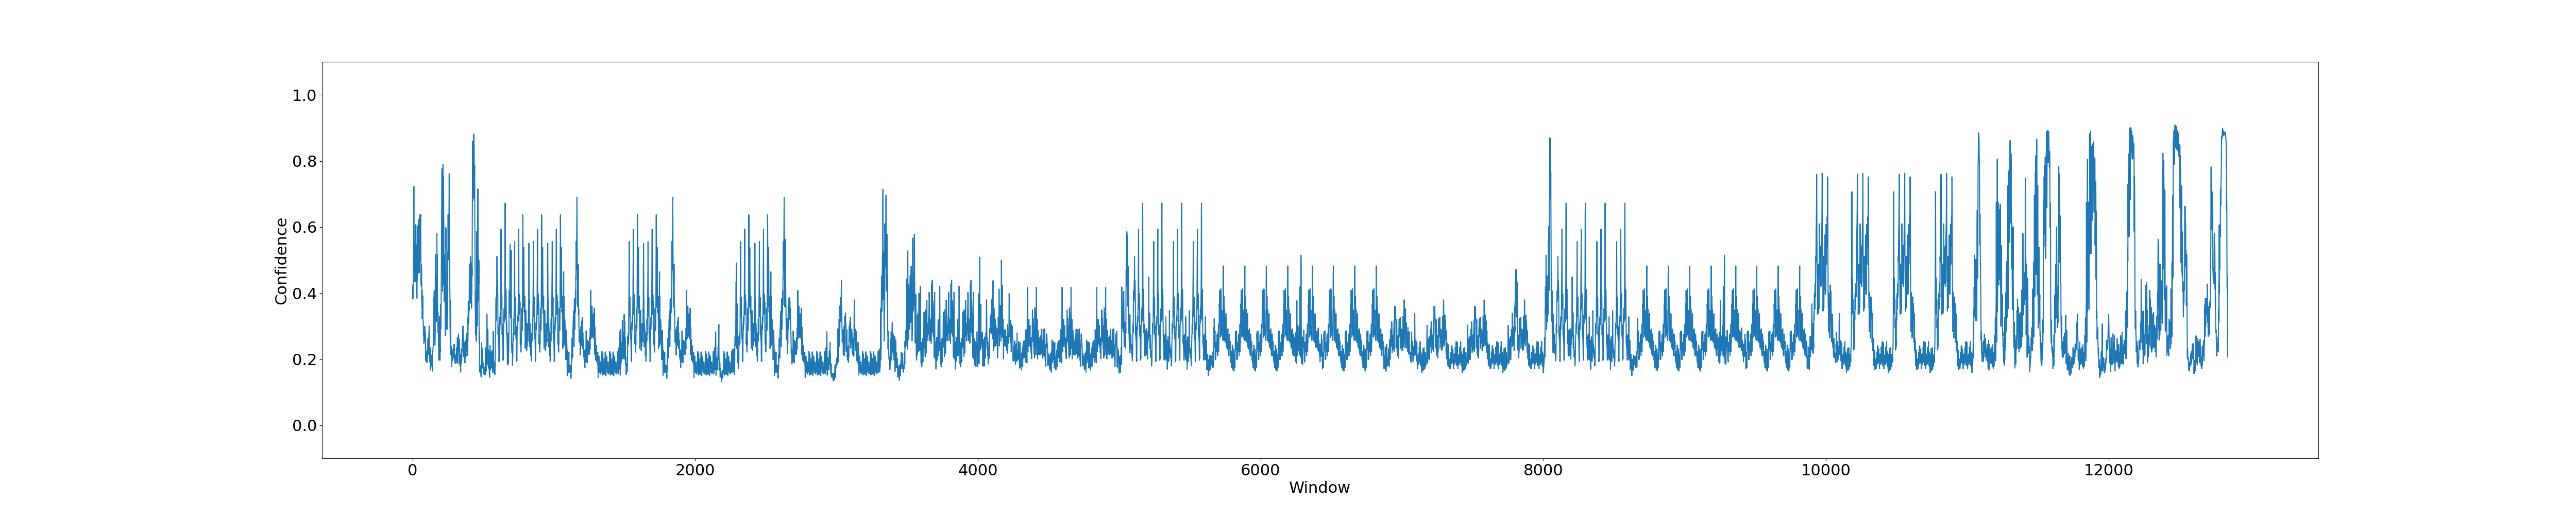
\includegraphics[scale=0.18]{../test_files/output_nosymbolic_FastSpec_wider/window50_overlap49_fig/testing_AES_CBC_nosymbolic.png}
			\caption{Confidence plot for AES-CBC.}
			\label{fig:conf-cbc}
		\end{subfigure}%
		\begin{subfigure}
			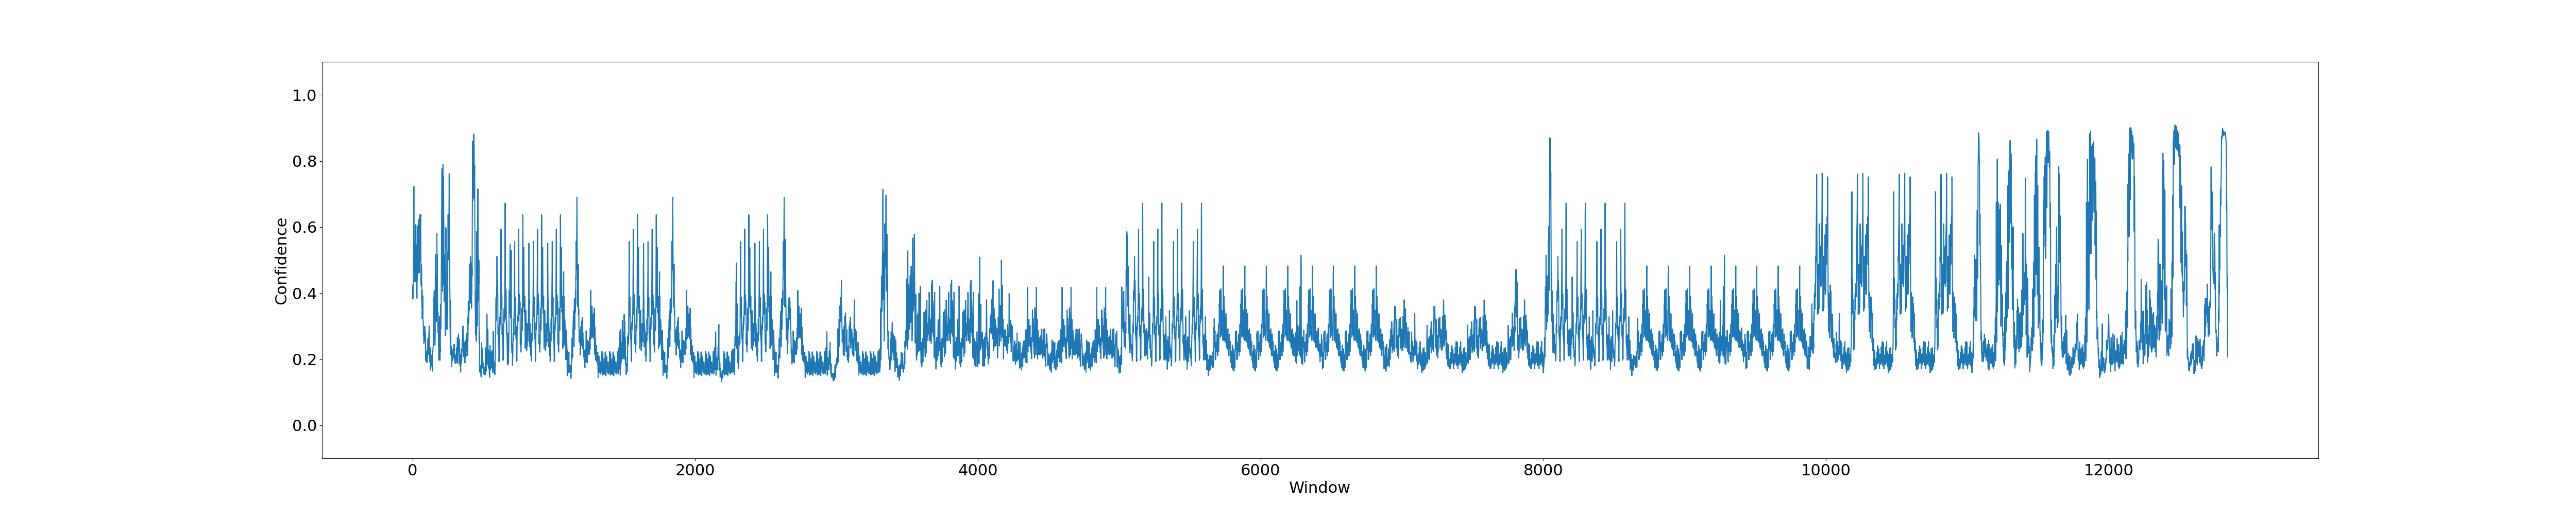
\includegraphics[scale=0.18]{../test_files/output_nosymbolic_FastSpec_wider/window50_overlap49_fig/testing_AES_CBC_nosymbolic.png}
			\caption{Confidence plot for AES-CTR.}
			\label{fig:conf-ctr}
		\end{subfigure}%
		\begin{subfigure}
			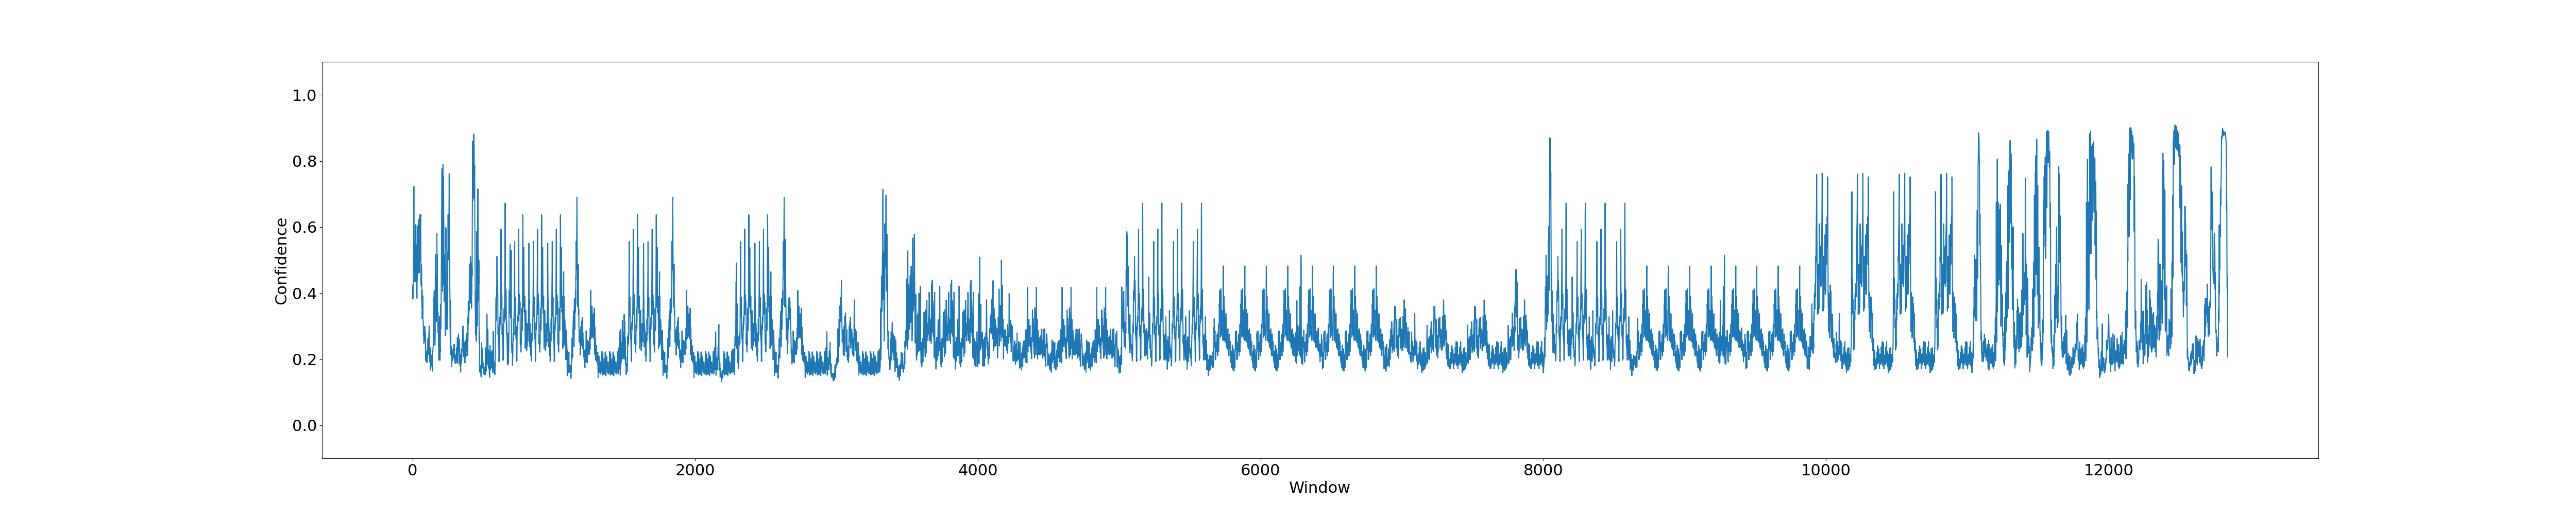
\includegraphics[scale=0.18]{../test_files/output_nosymbolic_FastSpec_wider/window50_overlap49_fig/testing_AES_CBC_nosymbolic.png}
			\caption{Confidence plot for AES-OFB.}
			\label{fig:conf-ofb}
		\end{subfigure}
	\end{figure}

\end{comment}

	\begin{figure}[!ht]
		\hspace*{-2.7cm}
		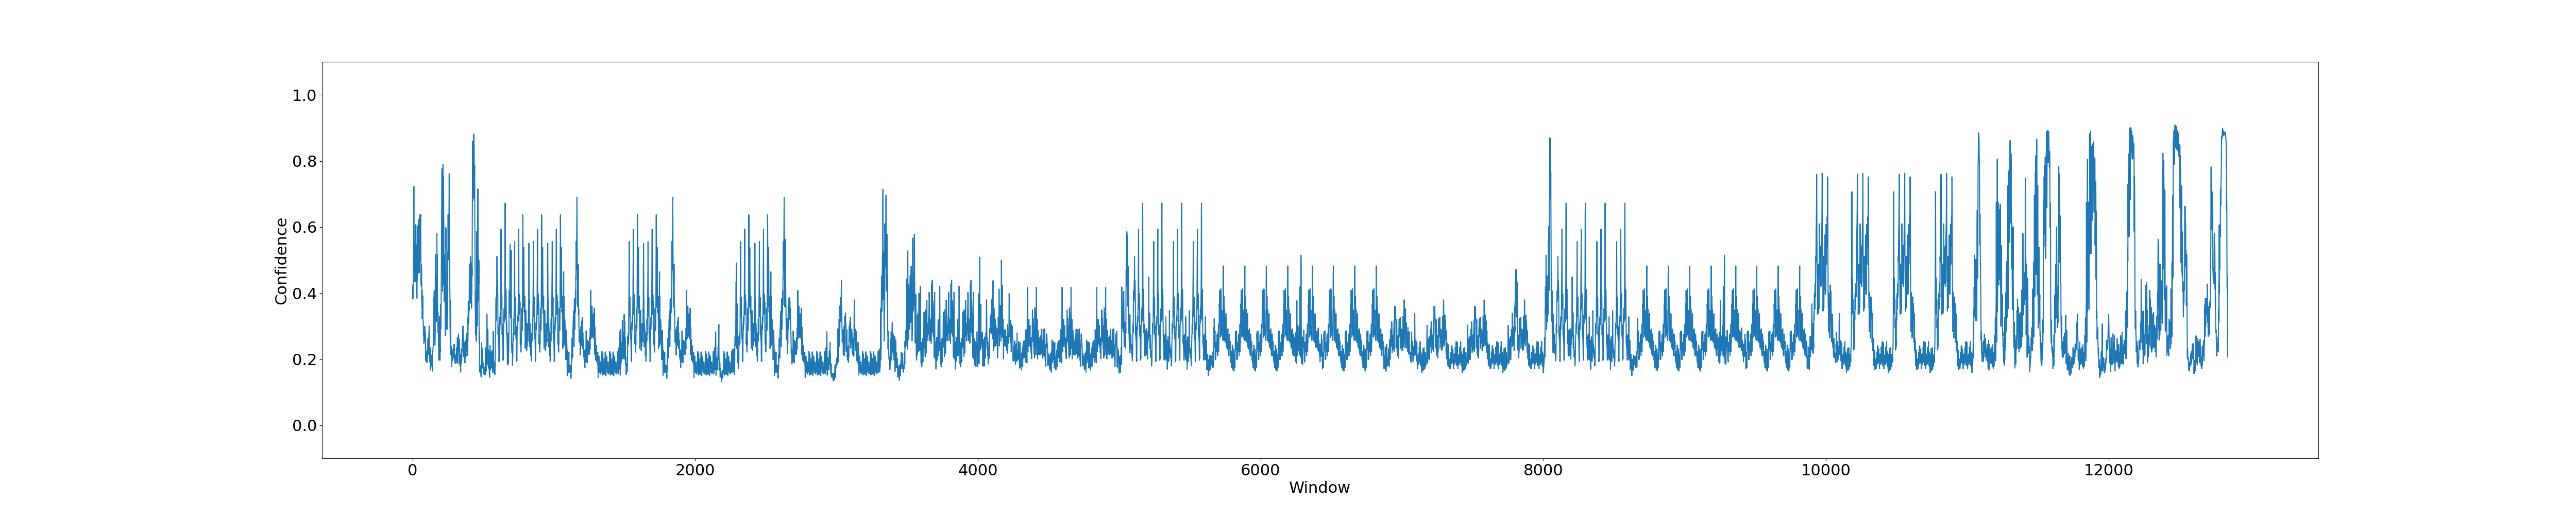
\includegraphics[width=1.3\textwidth]{../test_files/output_nosymbolic_FastSpec_wider/window50_overlap49_fig/testing_AES_CBC_nosymbolic.png}
		\caption{Confidence plot for AES-CBC.}
		\label{fig:conf-cbc}
	\end{figure}

	\begin{figure}[!ht]
		\hspace*{-2.7cm}
		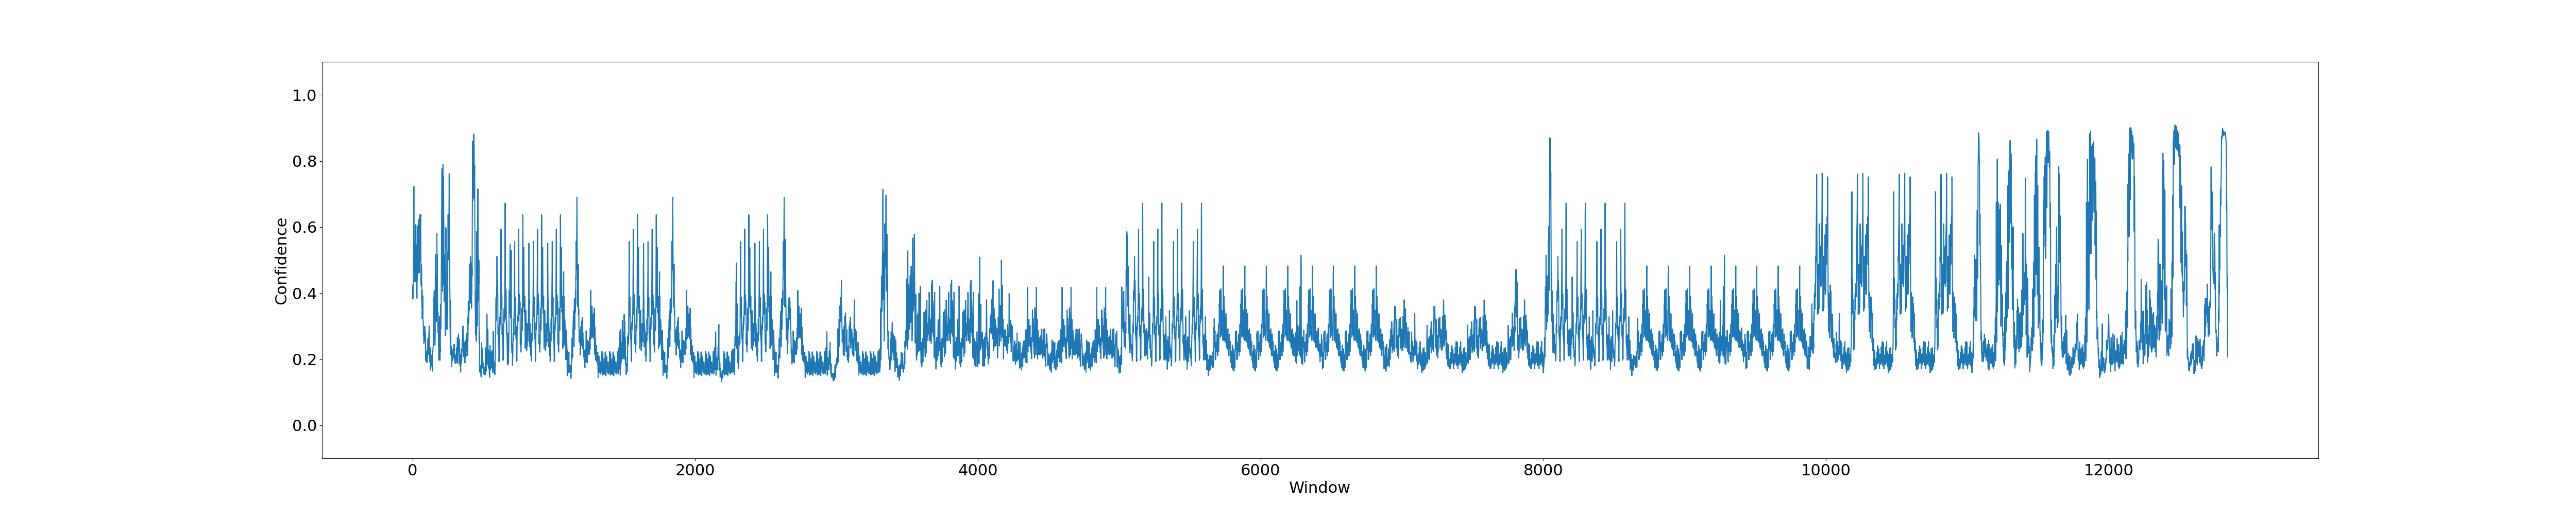
\includegraphics[width=1.3\textwidth]{../test_files/output_nosymbolic_FastSpec_wider/window50_overlap49_fig/testing_AES_CBC_nosymbolic.png}
		\caption{Confidence plot for AES-CTR.}
		\label{fig:conf-ctr}		
	\end{figure}

	\begin{figure}[!ht]
		\hspace*{-2.7cm}
		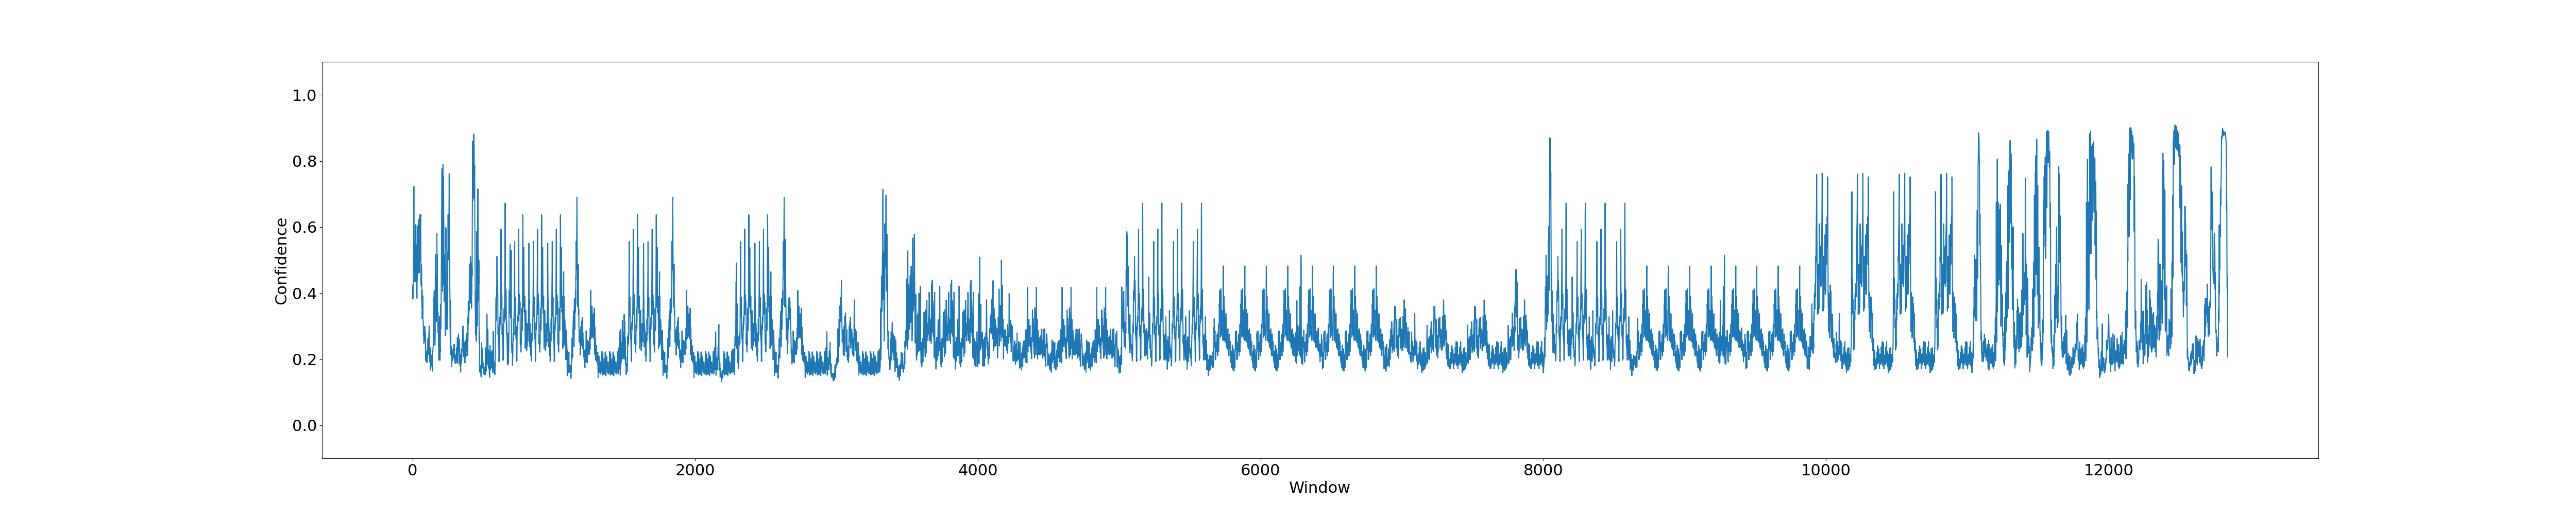
\includegraphics[width=1.3\textwidth]{../test_files/output_nosymbolic_FastSpec_wider/window50_overlap49_fig/testing_AES_CBC_nosymbolic.png}
		\caption{Confidence plot for AES-OFB.}
		\label{fig:conf-ofb}
	\end{figure}

	As we would expect, the plots look very similar, as they essentially execute the same algorithm with small variations.
	This confirm this impression, I wrote a Python script that overlaps the plots \ref{fig:conf-cbc} and \ref{fig:conf-ctr}: the result is shown in \ref{fig:overlap}. The two plots show uncanny similarities, even though there is a slight shift between them. To get a more satisfying figure, I manually fixed the difference of shift (for which it's sufficient to uncomment a specific line in the script), and obtained the plot \ref{fig:overlap-shifted}: we can see that the graphs overlap almost completely, apart from the a small section at the beginning and at the end.
	
	\begin{figure}[!ht]
		\hspace*{-1.5cm}
		\includegraphics[scale=0.5]{../imgs/overlap.png}
		\caption{Overlap between the confidence plot of AES-CBC and AES-CTR.}
		\label{fig:overlap}
	\end{figure}
	
	\begin{figure}[!ht]
		\hspace*{-1.5cm}
		\includegraphics[scale=0.5]{../imgs/overlap_shifted.png}
		\caption{Same overlap plot as \ref{fig:overlap}, but AES-CBC's confidence values have been shifted 50 units to left.}
		\label{fig:overlap-shifted}
	\end{figure}

	The same results can be obtained by overlapping different plots (i.e. AEC-CTR and AES-OFB, AES-CBC and AES-OFB), but I decided to omit the respective graphs for sake of brevity. However, those who are interested in reproducing the results, can modify the file \texttt{test\_files/overlap.py} and uncomment specific lines that I marked in the source code to make further verifications. To give a more formal proof of similarity, I also computed the Pearson's correlation coefficient (see Appendix \ref{appendix:maths}) on each pair of signals, obtaining:
	\begin{itemize}
		\item Correlation between AES-CBC and AES-CTR: 0.566
		\item Correlation between AES-CBC and AES-CTR: 0.519
		\item Correlation between AES-CBC and AES-CTR: 0.701
	\end{itemize}
	The outcome shows a moderate positive correlation, which is stronger between AES-CTR and AES-OFB, and thus confirms the similarity between the signals. These results can be reproduced by running the script \texttt{text\_files/overlap.py}.
	
	Due to the great level of similarity between the plots, I decided to analyse only one of three modes of operations taken into account, so I randomly chose AES-OFB. I will consider as potentially vulnerable only those windows that are assigned by FastSpec to a probability value greater than 80\% of being vulnerable to Spectre. To isolate such windows, I used another script, \texttt{test\_files/filter\_spectre\_wnd.py}, to filter out all the confidence values that are greater than 0.8 and then retrieve the corresponding lines of code from the \texttt{.tsv} file. For instance, for AES-OFB we obtained the line indexes shown in Figure \ref{fig:idx}. By grouping together contiguous values, we can extract from this list 6 sets of windows; finally, after re-arraging these windows according to Assembly's 
	syntax, we obtain the code snippets shown in the listing below: these are the pieces of code that FastSpec evaluated as likely to be subject to Spectre vulnerabilities.
	
	\begin{figure}[!ht]
		\centering
		\includegraphics[scale=0.5]{../imgs/vuln_indexes}
		\caption{The list of line indexes that correspond to vulnerable code snippets in the file \texttt{testing\_AES\_OFB\_nosymbolic.tsv}.}
		\label{fig:idx}
	\end{figure}

	These results are hard to interpret: FastSpec only points at fragments of Assembly language that may be vulnerable to Spectre, but without a reference to the source code, figuring out whether these instructions present at least the pattern of a Spectre gadget or not is definitely a challenge. One way around this problem would be disassembling the code, namely applying an algorithm that performs the inverse transformation of the assembler: in this way, we could obtain the high-level code that translates to that Assembly snippet. However, in this case a straightforward disassembly is not possible, as some tokens have been substituted with special markers (\texttt{<label>}, \texttt{<imm>}, \texttt{<UNK>}). If we give up the idea of disassembling the code, we can simply try to analyse the results as they are, comparing them with the gadgets published in \cite{Kocher2018}, where they are listed both in C and in Assembly.
	
	As mentioned in \cite{Tol2021}, the version of FastSpec that I used is able to recognise only Spectre-PHT (aka Spectre v1) vulnerabilities. To detect more variants, one should accomplish the following steps:
	\begin{enumerate}
		\item modify the mutational fuzzing algorithm to create gadgets of a specific variant;
		\item re-train SpectreGAN on the dataset generated in the previous point;
		\item re-train FastSpec on the new dataset to recognise that variant.
	\end{enumerate}
	Unfortunately, the authors of FastSpec did not publish the mutational fuzzing algorithm in any public repository, so this first issue prevents us for carrying out the whole process. Besides this, the training of GANs is notoriously slow: due to lack of time  therefore I decided to stick with the trained version 
		
	\begin{minipage}{.45\textwidth}
		\begin{lstlisting}[basicstyle=\footnotesize\ttfamily, caption={Window 369-379}, label=gadget1]
... %rdi
push %rdi
mov %rax , %rdi
callq <label> <imm> , %rsp
nop
leaveq
retq <UNK>
push %rbp
mov %rsp , %rbp
mov %rdi , <imm> ( %rbp )
mov %esi , <imm> ( %rbp )
mov %rdx , <imm> ( %rbp )
movl <imm> , <imm> ( %rbp )
cmpq <imm> , <imm> ( %rbp )
je cmpq <imm> ...
		\end{lstlisting}
	\end{minipage}\hfill
	\begin{minipage}{.45\textwidth}
		\begin{lstlisting}[caption={Window 7992-7997}, label=gadget2, numbers=right]
mov <imm> (%rbp), %edx
mov %dl, (%rax)
nop
pop %rbp
retq <UNK>
push %rbp
mov %rsp, %rbp
mov %rdi, <imm>(%rbp)
mov %rsi, <imm>(%rbp)
mov %rdx , <imm>(%rbp)
mov <imm>(%rbp), %rax
		\end{lstlisting}
	\end{minipage}

	\begin{minipage}{.45\textwidth}
	\begin{lstlisting}[caption={Window 11024-11031}, label=gadget3]
mov <imm> (%rbp), %edx
mov %dl, (%rax)
nop
pop %rbp
retq <UNK>
push %rbp
mov %rsp, %rbp
sub <imm>, %rsp
mov %rdi, <imm>(%rbp)
mov %rsi, <imm>(%rbp)
mov %rdx, <imm>(%rbp)
mov %rcx, <imm>(%rbp)
	\end{lstlisting}
\end{minipage}\hfill
\begin{minipage}{.45\textwidth}
	\begin{lstlisting}[basicstyle=\footnotesize\ttfamily, caption={Window 11351-11392}, label=gadget4, numbers=right]
mov <imm> (%rbp), %esi
mov <imm> (%rbp), %rax
add %rsi, %rax
xor %rcx, %rdx
mov %rdx, (%rax)
addl <imm>, <imm>(%rbp)
cmpl <imm>, <imm>(%rbp)
jbe subq <imm>, <imm>(%rbp)
addq <imm>, <imm>(%rbp)
addq <imm>, <imm>(%rbp)
cmpq <imm>, <imm>(%rbp)
ja movl <imm>, <imm>(%rbp)
cmpq <imm>, <imm>(%rbp )
je mov <imm>, (%rbp)
	\end{lstlisting}
\end{minipage}

	\begin{minipage}{.45\textwidth}
	\begin{lstlisting}[caption={Window 11598-11601}, label=gadget5]
mov <imm> (%rbp), %rax
mov %edx, (%rax)
nop
leaveq
retq <UNK>
push %rbp
mov %rsp, %rbp
sub <imm>, %rsp
mov %fs: <imm>, %rax
mov %rax, <imm>(%rbp)
xor %eax, %eax
movabs <imm>, %rax
movabs <imm>, %rdx
	\end{lstlisting}
\end{minipage}\hfill
\begin{minipage}{.45\textwidth}
	\begin{lstlisting}[basicstyle=\footnotesize\ttfamily, caption={Window 11868-11902}, label=gadget6, numbers=right]
mov %r12d, %edi
callq <label> <imm>, %rbx
cmp %rbx, %rbp
jne add <imm>, %rsp
pop %rbx
pop %rbp
pop %r12
pop %r13
pop %r14
pop %r15
retq <UNK>
nopw <UNK>
retq <UNK>
sub <imm>, %rsp
add <imm>, %rsp
	\end{lstlisting}
\end{minipage}
	\vspace{3mm}
	
	As described in Section \ref{sec:spectre-pht}, a Spectre-PHT attack needs a conditional branch to be carried out: this translates into a jump instruction in Assembly (e.g. \texttt{jmp}, \texttt{jbe}, \texttt{jae}). However, only 3 out of 6 detected gadgets present a jump instruction, namely listings \ref{gadget1}, \ref{gadget4}, and \ref{gadget6}, so it would be interesting to understand why FastSpec gave such high confidence values to the other snippets. 
	
	Besides this, being unable to go back at the source code is an important issue: it prevents us from understanding whether the jumps involve a user-controlled variable or not (and thus, if the variables used in the conditional expression can be manipulated by the attacker to cause a misprediction) and is also makes it infeasible to figure out whether the data that is loaded during the misprediction is sensible or not. 
	
	\subsection{Considerations about the results}\label{sec:final}
	Both tools tested in this work are restricted to detect Spectre v1 vulnerabilities. However, while \textsc{KLEESpectre} would probably require a total review of its design to make it suitable to spot different variants, FastSpec would only need to be re-trained on a dataset of different Spectre gadgets. 
	
	Among all the static analysers built to detect Spectre, \texttt{KLEESpectre} is certainly one of the most user-friendly: given a C program, it is sufficient to compile both the libraries and the program into LLVM bitcode and then run \textsc{KLEESpectre} on the result. The results, however, were mostly false positives: only in one case the code snipped pointed by the tool had all the characteristics of an actual Spectre v1 gadget. I noticed that \texttt{KLEESpectre} is not able to distinguish between a conditional branch and a cyle, as both these structures are encoded by branches (\texttt{br}) in the LLVM bitcode: this is a extensive source for false positives. Correcting this flaw should not be difficult: listings \ref{branch-ex} and \ref{cycle-ex} show (in a simplified syntax) a distinctive feature that should be considered when looking for Spectre gadgets.
	
	\begin{minipage}{0.45\textwidth}
	\begin{lstlisting}[basicstyle=\scriptsize\ttfamily, caption={\small LLVM bitcode fragment a conditional branch\vspace{2mm}}, label=branch-ex]
L0:	
	%cmp = < value >
  	br i1 %cmp, label %L1, label %L2
	...
L1:
  	< if_then body >
...
L2:
  	< if_else body >
...
	\end{lstlisting}
	\end{minipage}\hfill
	\begin{minipage}{0.45\textwidth}
	\begin{lstlisting}[basicstyle=\scriptsize\ttfamily, caption={\small LLVM bitcode fragment encoding a cycle\vspace{2mm}}, numbers=right, label=cycle-ex]
L0:
 	%cmp = < value >
 	br i1 %cmp, label %L1, label %L2
  	...
L1:
  	< cycle body >
  	br label %L0	// this branch!
L2:
  	< outer body >
...
	\end{lstlisting}
	\end{minipage}
	\vspace{3mm}
	
	Line 7, in the listing on the right, is the elements that would allow \textsc{KLEESpectre} to figure out that what is analysing is not a conditional branch, but a cycle.
	
	Some results still remain unclear, for example when the Spectre gadget was identified in two different, unrelated files: a much more detailed analysis of the design of the tool would be necessary to understand where does this issue come from.
	\paragraph{}Despite the encouraging premises provided in the paper \cite{Tol2021}, FastSpec gave disappointing results: only 50\% percent of the alleged gadgets presented a jump, a primary condition for a Spectre v1 vulnerability. Unfortunately, without any kind of annotation that allows to link the alleged gadgets to pieces of the source code, it's difficult to evaluate the quality of the results. 
	
	\chapter{Conclusions}\label{conclusions}
	
	This work was motivated both by the curiosity of understanding more about one of the most serious flaws in modern processors and by the interest in discovering how static analysis can be applied. At the beginning of this work, I asked three research questions and I tried to investigate them with the instruments at my disposal. In this conclusive chapter, I would like to summarize the answers that I found (?) and discuss what improvements could be made.
	\paragraph{} The first question was:
	\begin{quote}
		\textit{Do FastSpec and KLEESpectre detect any Spectre vulnerability in the AES implementation?}
	\end{quote}
	The answer has already been discussed in the final section of Chapter \ref{chapter:verification}, but here I summarize the main observations. Both tools indeed found some alleged vulnerabilities, but a careful analysis revealed that most of them are false positives. More precisely, only one snippet, identified by \textsc{KLEESpectre}, has all the characteristics of a Spectre gadget and is potentially exploitable. FastSpec's output, instead, didn't provide enough information to evaluate the quality of the detected gadgets. 
	
	\paragraph{} The second question was formulated as follows:
	\begin{quote}
		\textit{Do FastSpec and KLEESpectre provide the same results?}
	\end{quote}
	This question is difficult to tackle, as the two tools provided outputs in different formats: \textsc{KLEESpectre} performed the analysis on LLVM bitcode, while FastSpec operated on Assembly code (AT\&T syntax). For this reason, we cannot establish an immediate relationship between the snippets detected as vulnerable. (...) 
	
	\paragraph{} The third question is stated as follows:
	\begin{quote}
		\textit{Comparing the results obtained on AES in its OpenSSL v1.0.02 implementation (last revised in 2015, before the discovering of Spectre) in its OpenSSL v3.0.03 implementation (the latest version), are there any differences?}
	\end{quote}
	The motivation for this question was to verify whether OpenSSL developers ...
	To answer this question, I relied on \textsc{KLEESpectre output}, as I found it easier to interpret, I could observe that the only exploitable gadget detected in version 1 was indeed removed in version 3. 
	
	\section{Possible improvements}
	Despite the many points discussed in this thesis, there is certainly still room for further work and improvements. First, it would be interesting to test the presence of other Spectre variants on OpenSSL cryptographic libraries: a natural way to do this would be to use more "powerful" tools, namely tools that are designed to cover more variants. However, it would be interesting to see how \textsc{KLEESpectre} and FastSpec could be extended to improve their detection capabilities. 
	
	Moreover, throughout this thesis I always talked about \textit{alleged} vulnerabilities, not only because many gadgets were evidently false positives, but also because not all gadgets are exploitable. Most of the software we use every day contains various flaws that can be \textit{technically} be classified as security issues; however, most of them are infeasible to exploit or do not endanger sensible information. In order to claim that OpenSSL libraries have a Spectre vulnerability, we should try to run a proper Spectre attack on the target and see if it is successful.
	
	\section{Possible improvements}
	
	\appendix
	
	\chapter{Mathematical notions}\label{appendix:maths}
	\section{Pearson's coefficient}
	Pearson's correlation coefficient \cite{Pearson1895} is a measure of linear correlation between two sets of data. The value of the coefficient ranges in the interval $[-1,+1]$: values close to -1 indicate a \textit{negative} (or "inverse") correlation between the two variables, meaning that greater values of variable $X$ correspond to lower values of variable $Y$. On the other hand, values close to +1 indicates a \textit{positive} (or "direct") correlation, meaning that greater values of $X$ correspont to greater values also in $Y$. A coefficient of 0 indicates no correlation between the two variables.	
	
	Mathematically, given two sets of values $X$ and $Y$, the Pearson's correlation coefficient is computed as follows:
	\[
		r = \frac{\sum_i(x_i-\bar{x})(y_i-\bar{y})}{\sqrt{\sum_i(x_i-\bar{x})^2\sum_i(y_i-\bar{y})^2}}
	\]
	where $x_i\in X$, $y_i\in Y$, $\bar{x}$ is the mean of the values in $X$, and $\bar{y}$ is the mean of the values in $Y$. 
	
	In order to compute the Pearson's correlation coefficient, the two datasets should satisfy the following requirements:
	\begin{itemize}
		\item both sets express \textbf{quantitative} properties: with reference to FastSpec results, confidence is a quantitative value, as it measures the \textit{amount} of confidence the tool has in claiming that a piece of code contains a vulnerability;
		\item the data is \textbf{normally distributed};
		\item the data have \textbf{no outliers}, i.e. it contains are no observations that don’t follow the same patterns as the rest of the data;
		\item the relationship is \textbf{linear}, meaning that the relationship can be described reasonably well by a linear function.
	\end{itemize}

	Visually, the correlation coefficient can be seen as a measure of how close the data point are to a line of best fit. Consider \ref{fig:pearson}: the top left plot shows a strong positive correlation, in fact the points are closer to the linear function that represents the line of best fit. The top right plot, instead, shows a situation of no correlation, where the points are placed randomly in the space with respect to the line.

	\begin{figure}[!ht]
		\centering
		\includegraphics[scale=0.4]{../imgs/pearson_coefficient2.png}
		\captionsetup{width=0.7\textwidth}
		\caption{Pearson's Correlation Coefficient, $r$ (Credits to: \href{https://statistics.laerd.com/statistical-guides/pearson-correlation-coefficient-statistical-guide.php}{Laerd Statistics}). The horizontal axis corresponds to values in the set $X$, while the vertical axis is for values in $Y$.}
		\label{fig:pearson}
	\end{figure}
	
	\chapter{Deep Learning}\label{appendix:dl}
	\section{Generative Adversarial Networks (GANs)}
	The Generative Adversarial Network \cite{Goodfellow2014} is a learning framework designed for the task of \textit{generative modelling}, an unsupervised learning task that involves the automatic discovering and learning of patterns in data distributions in such a way that the model can generate new examples that plausibly could have been drawn from the original data set. The innovative idea behind GANs lies in the learning strategy, that sees two actors involved:
	\begin{itemize}
		\item a \textbf{Generative} net, $G$, that generates data;
		\item a \textbf{Discriminator} net, $D$, that evaluates these data.
	\end{itemize}
	Intuitively, the Discriminator should be able to distinguish authentic data from artificially generated data. The goal of the Generator is to produce, starting from a random data distribution, increasingly better data that will eventually fool the Discriminator. From a game theory point of view, the convergence of a GAN is reached when the generator and the discriminator reach a \textit{Nash equilibrium} \cite{Ratliff2013}.
	\paragraph{Generator}
	To produce a certain kind of data, we assume that there exists a probability distribution (referred to as \textbf{target distribution}, $p_t$) that describes that data we want to create: the points of the distribution represent vectors of features that characterize that type of data. The goal of the Generator is to be able to sample a random noise, $z$, from a normal or uniform distribution (denoted by $p_g$) and turn it into a point $x$  following the target distribution, through a function denoted by $Gen()$:
	\[
	x = Gen(z) \text{ with } z \sim p_g
	\]
	
	Conceptually, $z$ represents the latent features of the images generated, for example, the colour or the shape. In fact, the space from which the Generator samples the seed z is also referred to as \textbf{latent space}.
	\paragraph{Discriminator}
	The Generator, alone, can only produce some random noise: the purpose of the Discriminator is to guide the Generator to create data that look more similar to the real ones. It's fundamental to underline that before the beginning of the adversarial exchange between the two nets, the Discriminator must be trained (in a supervised fashion) with a data set of real and fake data.
	For each point in the training set, the net outputs the value $D(x)$, representing the probability that $x$ is real. Thus, what we \textit{ideally} want to obtain at the end of the training is that:
	\[
	D(x) = \begin{cases}
		1 &\text{ if the input is real }\\
		0 & \text{ otherwise }
	\end{cases}
	\]
	Concretely, during the training, the goal is to \textit{maximize} the ability of discerning real data from fake ones:
	\[
	\max_D V(D) = \mathbb{E}_{x\sim p_t(x)}[\log D(x)] + \mathbb{E}_{z\sim p_z(z)}[1-(\log D(G(z)))]
	\]
	where $\mathbb{E}$ denotes the expected value.
	
	To measure the loss, it is possible to use \textbf{cross-entropy}, the most popular loss function for learning algorithms that use gradient descent.
	\paragraph{Adversarial learning}
	Once the Discriminator is properly trained, the Generator enters into play, and the adversarial confrontation begins. The goal of the Generator is to minimize the difference between the data it generates and real data:
	\[
	\min_G V(G) = \mathbb{E}_{z\sim p_z(z)}[\log(1-D(G(z)))]
	\]
	Overall, the two nets play a so-called \textbf{minimax game}:
	\[
	\min_G \max_D V(D,G) = \mathbb{E}_{x\sim p_t(x)}[\log D(x)] + \mathbb{E}_{z\sim p_z(z)}[\log (1-D(G(z)))]
	\]
	where $V(D,G)$ represents the value function.
	
	The last equation makes it clear why this style of training is called \textit{adversarial}: while the Generator tries to minimise a function, the Discriminator tries to maximise it, thus the two networks have opposite goals.
	
	\section{Bidirectional Encoder Representations from Transformers (BERT)}
	BERT \cite{Devlin2018} is a deep learning technique for Natural Language Processing (NLP) proposed by Google in 2018. The goal of this framework is to "learn a language" by understanding of how words fit into different contexts. It's interesting to reflect upon how this mechanism resembles the way non-native speakers learn the meaning of particular words in a new language: it is well known that certain expressions don't have a faithful translation in other languages. For this reason, non-native speakers learn what these words stand for simply by observing in what context they are used and what emotional characterisation they are accompanied by. A similar idea applies also to BERT, that uses transformers (described in the next section) to accomplish this task.
	
	\subsection{Transformers}
	Transformers \cite{Vaswani2017} were introduced in 2017 by a team at Google Brain to improve certain limitations of recurrent neural networks (RNNs), such as LSTMs. The typical architecture is depicted in Figure \ref{fig:transformer}.
	\begin{figure}[!ht]
		\centering
		\includegraphics[scale=0.4]{../imgs/transformers}
		\captionsetup{width=.7\linewidth}
		\caption{Transformers architecture (source: \cite{Vaswani2017}). On the left side there is the encoder, while on the right there is the decoder.}
		\label{fig:transformer}.
	\end{figure}
	
	\paragraph{Input processing}
	Transformers are typically used for machine translation tasks. For this reason, the input is usually a sentence, namely a set of words, that need to be converted in a mathematical representation in order to be processed by the network. The sentence in a language $\mathcal{L}_1$ is thus passed to the Input Embedding layer, which produces a \textit{vector embedding} for each word. Vector embeddings are a common way to represent words, that tend to assign close vectors to words that have a similar meaning. However, this representation is not enough: as we said in previously in this section, the meaning of a words depends also from the context in which it is placed. For this reason, the vector embeddings are combined with a Positional Encoding, namely a vector that gives context based on the position of the word in a sentence. 
	
	After this processing, we obtain a vector representation of the initial sentence that takes into consideration not only the meaning of a words, but also the context in which it appears.
	\paragraph{Encoder}
	Once the input processing phase is completed, the vectors are passed to the encoding block, whose goal is learn the characteristics of the source language and the context of a sentence. The encoder consists in two main units:
	\begin{enumerate}
		\item a \textbf{Multi-head Attention} layer, that computes an attention vector for each word of the sentence: assuming that the sentence contains $n$ words, the attention vector for the $i$-th word is an $n$-dimensional vector, where the $j$-th coefficient represents how important the $j$-th words is to determine the meaning of the $i$-th word;
		\item a \textbf{Feed-Forward} layer, that is applied to each attention vector, in order to transform them in a way that is more easy to process for the decoder block.
	\end{enumerate} 
	
	\paragraph{Decoder}
	The decoder is feed with the translation of the sentence that was given in input to the encoder and the same processing steps are performed to transform the sentence into its most accurate mathematical representation. The decoder block has then three main components:
	\begin{enumerate}
		\item a \textbf{Masked Multi-head Attention} layer, that masks those words in the destination language that haven't been translated. To understand why this layer is necessary, remember that, when we train a transformer, we have at our disposal (1) a whole sentence in the source language (that is fed into the encoder) and (2) the whole translation of the original sentence in the destination language (that is provided to the decoder). To generate the $i$-th word in the destination language, the transformer it is allowed to use (1) \textit{all} the words from the input sentence but (2) \textit{only} the $(i-1)$ previous words of the sentence in the destination language! For this reason, all the words from position $i$ onwards are "masked", i.e. are substituted with a special token (usually \texttt{<MASK>}).
		\item a \textbf{Multi-head Attention} layer, which takes in input (1) the embedding vectors produced by the encoder and (2) the attention vectors produced by the previous layer of the decoder. The output is a vector where each coefficient expresses how the corresponding word relates to the other elements of the sentence, both in the source and in the destination language.
		\item a \textbf{Feed-Forward} layer, that has the same purpose as the one in the encoder block.
	\end{enumerate}
	The output of the decoder is a vector of probabilities: the $i$-th coefficient corresponds to the probability that the $i$-th words is the next word in the translated sentence.
	\subsection{Architecture}
	As we said in the previous section, the two block of a transformer accomplish different functions:
	\begin{itemize}
		\item the \textbf{encoder} learns what is the source language and what is context;
		\item the \textbf{decoder} learns how to map words in the source language into words of the destination language.
	\end{itemize}
	BERT was designed to solve problems (such as sentiment analysis, question answering, text summarisation, etc.) that have to do with understanding language and context, while the translation part is irrelevant. Therefore, BERT's architecture is just made by a stack of encoders.

	\subsection{Training}
	The training phase consists in two parts: \textit{pre-training} and \textit{fine-tuning}. The first part is needed to make BERT learn what is language and what is context. Once this phase is completed, we must to fine-tune our model to accomplish a specific task, for example sentiment analysis. 
	
	\paragraph{Pre-training} Firstly, BERT is trained on two unsupervised task simultaneously: Masked Language Model (MLM) and Next Sentence Prediction (NSP). Note that these tasks are not BERT's final goal! These tasks are only needed to make BERT understand the language, but the training on the objective task will be made only during the fine-tuning phase.
	During the MLM task, we provide BERT with sentences where random words have been masked and the network must learn to guess the correct word in each place. In order to succeed, BERT is forced to learn the notion of context \textit{within the same sentence} and to evaluate whether a word can fit into a given context or not. For the NSP task,  BERT receives in input two sentences with a temporal connection, meaning that one of the two sentences only makes sense when placed before or after the other (for example, when reading $A =$ "This is John" and $B =$ "He is my friend", we can immediately see that $B$ makes sense only if it's preceeded by $A$). BERT must learn to figure out what sentence comes after the other one: in this way it comprehends context even \textit{across different sentences}.
	\paragraph{Fine-tuning} Once BERT has been sufficiently trained, we can fine-tune it to accomplish a more specific task, for instance:
	\begin{itemize}
		\item classification tasks such as \textbf{sentiment analysis}, which is done similarly to the NSP task.
		\item \textbf{question answering}...
		\item ...
	\end{itemize}
	
	\chapter{Block ciphers and AES}\label{appendix:aes}
	The goal of this appendix is to provide the basic notions concerning block ciphers and modes of operations that are fundamental to understand how AES works. Given the breadth of the topic, here we will discuss only the concepts that are strictly necessary to understand the core of this thesis, but the curious readers can rely on the references given in the rest of the appendix to dig deeper into the topic.
	
	The appendix begins by presenting some game-based security notions (maybe not), necessary to understand how the security of ciphers is evaluated. Then we briefly describe block ciphers in Section \ref{sec:block-ciphers}, before proceeding with Section \ref{sec:modes}, where we present how a block cipher can be used repeatedly on different part of the message to produce the final encryption. Finally, we have all the tools to reach Section \ref{sec:aes}, concerning the history and the design of AES.
	
	\section{Block ciphers}\label{sec:block-ciphers}
	A block cipher is a deterministic algorithm $F$ that operates on data units of fixed length, called \textit{blocks}. $F$ accepts in input a data block of size $n$, and performs a transformation using a key $k$, producing in output a block of same size as the input. More formally, $F$ is defined as follows:
	\[
		F: \{0,1\}^{|k|} \times \{0,1\}^n \rightarrow \{0,1\}^n
	\]
	where $|k|$ represents the key length and $n$ the size of the block. The definition given above means that a ciphertext $c$ is obtained from a key $k$ and a message $m$ (also called "plaintext") as:
	\[
		F(k,m) = c
	\]
	Since the key remains fixed for a certain number of encryptions, before being refreshed, we can parametrise $F$ on $k$, defining $F_k(m) \defeq F(k,m)$.
	
	If $F$ represents the encryption algorithm, then the decryption algorithm is obtained simply by computing $F^{-1}$, thus:
	\[
		F^{-1}(k,c) = m
	\]

	\section{Modes of operation}\label{sec:modes}
	There is a clear limitation of block ciphers: they can only encrypt data of fixed size. While the case in which $|m| < n$ can be easily circumvented through padding, if $|m| > n$ we would be forced to discard a part of the message. \textit{Modes of operation} address this problem, providing a way to securely and efficiently encrypt long messages using block ciphers. In simple terms, a mode of operation defines how to concatenate the use of a block cipher in such a way that each cipher encrypts a specific part of the message. In general, if the message has size $|m| > n$, then $m$ is split in $\ell = \frac{|m|}{n}$ different blocks, $m_1$, $m_2$, ... , $m_{\ell}$, and the whole ciphertext is obtained as:
	\[
	c = \langle F(k, m_1), F(k, m_2), ..., F(k, m_{\ell})\rangle
	\]
	where the operator $\langle \cdot , ..., \cdot \rangle$ represents a a generic combination. For the sake of brevity, the rest of this section will present only the modes of operation that were tested in this thesis. Those who are interested in other modes can find them in the references provided throughout this Appendix.

	\subsection{Cipher Block Chaining (CBC) mode}
	To encrypt using this mode, we choose uniformly at random an initialization vector ($IV$) of length $n$, which is unique for every encryption. Then, we generate the ciphertext blocks by applying the block cipher to the XOR of the current plaintext block and the previous ciphertext block. Figure \ref{fig:cbc} visually depicts the process.
	\begin{figure}[!ht]
		\centering
		\includegraphics[scale=0.4]{../imgs/cbc}
		\captionsetup{width=.7\linewidth}
		\caption{Visual representation of Cipher Block Chaining (CBC) mode (source: \cite{Katz2007})}
		\label{fig:cbc}
	\end{figure}
	Mathematically, the ciphertext is the result of the following operations:
	\[
	\begin{cases}
		c_1 = F_k(IV \oplus m_1)\\
		c_i = F_k(c_{i-1}\oplus m_i) \text{ for all } i>1
	\end{cases}
	\]
	Using a random initialisation vector introduces an element of randomness in the encryption process and makes it not deterministic: the repeated encryption of the same plaintext results in different ciphertext. 
	We will not dive into the discussion about the security of modes of operations, as it is beyond the scope of this appendix. However, it's sufficient to mention that introducing an element of randomness during the encryption ensures to a greater level of security with respect to deterministic schemes. Clearly, the choice of the $IV$ plays a crucial role: it should be chosen uniformly at random and it must be included in the ciphertext to allow a correct decryption.
	
	Despite being considered secure, this mode of operation presents a mild disadvantage: since the encryption of block $i$ depends on the value of the previous ciphertext, the computation of the final ciphertext can't be parallelised, thus it's not the most efficient choice.
 	\subsection{Output Feedback (OFB) mode}
 	The Output FeedBack (OFB) mode works similarly to the CBC mode, performing some operations in a different order. Figure \ref{fig:ofb} is a high-level depiction of how the OFB mode works.
 	\begin{figure}[!ht]
 		\centering
 		\includegraphics[scale=0.4]{../imgs/ofb}
 		\captionsetup{width=.7\linewidth}
 		\caption{Visual representation of Output Feedback (OFB) mode mode (source: \cite{Katz2007})}
 		\label{fig:ofb}
 	\end{figure}
 	This mode of operation, like Cipher Block Chaining, involves a random initialisation vector, whose value must be unpredictable to guarantee the minimum security requirements.
 	
 	Mathematically, the ciphertext is computed as follows:
 	\[
 	\begin{cases}
 		c_1 = F_k(IV) \oplus m_1\\
 		c_i = F_k(c_{i-1}) \oplus m_i \text{ for all } i>1
 	\end{cases}
 	\]
 	This mode of operation presents the same disadvantage of the CBC-mode, because the computation can't be parallelised.
	\subsection{Counter (CTR) mode}
	In the CTR mode of operation, a counter $ctr \in \{0,1\}^n$ is sampled uniformely at random. Then, the encryption unfolds as follows:
	\[
		c_i = F_k(ctr + i) \oplus m_1
	\]
	where $ctr$ and $i$ are viewed as integers and addition is done modulo $2^n$. Figure \ref{fig:ctr} depicts In contrast to all the modes discussed previously, the CTR mode has the advantage that encryption and decryption can be fully parallelised, since all the blocks can be computed independently of each other.
	\begin{figure}[!ht]
		\centering
		\includegraphics[scale=0.35]{../imgs/ctr}
		\captionsetup{width=.7\linewidth}
		\caption{Visual representation of Counter (CTR) mode mode (source: \cite{Katz2007})}
		\label{fig:ctr}
	\end{figure}
	
	\section{AES: Advanced Encryption Standard}\label{sec:aes}
	AES \cite{Katz2007} \cite{AES-FIPS} is a block cipher that was born in 1998 as replacement of the obsolete DES (Data Encryption Standard) \cite{DES1999}, on request of the U.S. government. At first, its use was limited to military purposes, but nowadays it’s one of the most common block ciphers in use, deeply embedded in various applications. 
	
	The AES cipher has a 128-bit block length and can use 128-, 192-, or 256-bit keys; depending on the key length, the algorithm performes 10, 12 or 14 rounds respectively. During the execution, AES works on a $4\times 4$ array of bytes, called \textit{state}, and each step of the algorithm performs a certain trasformation on this state. More precisely, the main operations present in the algorithm are:
	\begin{enumerate}
		\item \textsf{KeyExpansion}: Derives fresh 128-bit key at each round, using the AES key schedule.
		\item \textsf{AddRoundKey}: Combine each byte of the $4\times 4$ state matrix with a byte of the selected key using the XOR ($\oplus$) operation.
		\item \textsf{SubBytes}: Performs a non-linear substitution where each byte is replaced with another according to a lookup table.
		\item \textsf{ShiftRows}: Performs a transposition where the last three rows of the state are shifted cyclically of a certain number of steps.
		\item \textsf{MixColumns}: Performs a linear mixing operation which operates on the columns of the state, combining the four bytes in each column.
	\end{enumerate}
	Each operation is executed multiple times, according to the order represented in Algorithm \ref{alg:aes}. In this algorithm, we denote with $nRounds$ the number of rounds executed according to the key length, with $K$ the key derived from the AES key schedule at each round, with $S$ the state during each step of the execution, with $SBox$ the non-linear transformation performed during SubBytes, with $nRows$ the amount of shift in the ShiftRow operation, and with $m$ the invertible linear transformation used in MixColumns.
	\begin{algorithm}[H]
		\caption{Advanced Encryption Standard (AES)}
		\label{alg:aes}
		\begin{algorithmic}[1]
			\For{$i=0$ to $nRounds-1$}
			\State $K$ $\leftarrow$ KeyExpansion()
			\State $S$ $\leftarrow$ AddRoundKey($K$)
			\State $S$ $\leftarrow$ SubBytes($Sbox$)
			\State $S$ $\leftarrow$ ShiftRows($nRows$)
			\State $S$ $\leftarrow$ MixColumns($m$)
			\EndFor
			\State $S$ $\leftarrow$ SubBytes($Sbox$)
			\State $S$ $\leftarrow$ ShiftRows($nRows$)
			\State $S$ $\leftarrow$ MixColumns($m$)
		\end{algorithmic}
	\end{algorithm}
	\bibliography{thesis_ref}{}
	\bibliographystyle{acm}
\end{document}